         \chapter{Transverse pulses}
    \setcounter{figure}{1}
    \setcounter{subfigure}{1}
    \label{21d48a6f8839b4b265192acd9ea3d978}
    
    
    
    
       
         \section{ Introduction and key concepts}
    \nopagebreak
            \label{m38801} $ \hspace{-5pt}\begin{array}{cccccccccccc}   
\includegraphics[width=0.75cm]{col11305.imgs/summary_fullmarks.png} &   \end{array} $ \hspace{2 pt}\raisebox{-5 pt}{} {(section shortcode: P10037 )} \par 
    
    
    
    
    
    
  
    \label{m38801*cid2}
            \subsection{ Introduction}
            \nopagebreak
            
      
      \label{m38801*id312450}This chapter forms the basis of the discussion into mechanical waves. Waves are all around us, even though most of us are not aware of it. The most common waves are waves in the sea, but waves can be created in any container of water, ranging from an ocean to a tea-cup. Waves do not only occur in water, they occur in any kind of medium. Earthquakes generate waves that travel through the rock of the Earth. When your friend speaks to you he produces \textsl{sound waves} that travel through the air to your ears. Light is made up of electromagnetic waves. A wave is simply moving energy.\par 
    
    \label{m38801*cid3}
            \subsection{ What is a \textsl{medium}?}
            \nopagebreak
            
      
      \label{m38801*id312816}In this chapter, as well as in the following chapters, we will speak about waves moving in a medium. A medium is just the substance or material through which waves move. In other words the medium carries the wave from one place to another. The medium does not create the wave and the medium is not the wave. Therefore the medium does not travel with the wave as the wave propagates through it. Air is a medium for sound waves, water is a medium for water waves and rock is a medium for earthquakes (which are also a type of wave). Air, water and rock are therefore examples of media (media is the plural of medium).\par 
\label{m38801*fhsst!!!underscore!!!id51}\begin{definition}
	  \begin{tabular*}{15 cm}{m{15 mm}m{}}
	\hspace*{-50pt}  
\includegraphics[width=0.5in]{col11305.imgs/psflag2.png}   & \Definition{   \label{id2434692}\textbf{ Medium }} { \label{m38801*meaningfhsst!!!underscore!!!id51}
      \label{m38801*id312830}A medium is the substance or material in which a wave will move. \par 
       } 
      \end{tabular*}
      \end{definition}

      \label{m38801*id312841}In each medium, the atoms that make up the medium are moved \textsl{temporarily} from their rest position. In order for a wave to travel, the different parts of the medium must be able to interact with each other.\par 
    
    \label{m38801*cid4}
            \subsection{ What is a \textsl{pulse}?}
            \nopagebreak
            \label{m38801*secfhsst!!!underscore!!!id58}
            \subsubsection{  Investigation : Observation of Pulses }
            \nopagebreak
            
      \label{m38801*id312873}Take a heavy rope. Have two people hold the rope stretched out horizontally. Flick the rope at one end only once.\par 
      \label{m38801*id312879}
        
    \setcounter{subfigure}{0}


	\begin{figure}[H] % horizontal\label{m38801*id312882}
    \begin{center}
    \label{m38801*id312882!!!underscore!!!media}\label{m38801*id312882!!!underscore!!!printimage}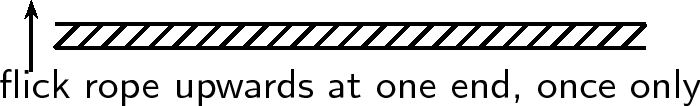
\includegraphics[width=300px]{col11305.imgs/m38801_PG10C4_001.png} % m38801;PG10C4\_001.png;;;6.0;8.5;
        
      \vspace{2pt}
    \vspace{.1in}
    
    \end{center}

 \end{figure}   

    \addtocounter{footnote}{-0}
    
      \par 
      \label{m38801*id312888}What happens to the disturbance that you created in the rope? Does it stay at the place where it was created or does it move down the length of the rope? \par 

      \label{m38801*id312898}In the activity, we created a \textsl{pulse}. A pulse is a \textsl{single} disturbance that moves through a medium. In a transverse pulse the displacement of the medium is perpendicular to the direction of motion of the pulse. Figure~6.2 shows an example of a transverse pulse. In the activity, the rope or spring was held horizontally and the pulse moved the rope up and down. This was an example of a transverse pulse.\par 
\label{m38801*fhsst!!!underscore!!!id71}\begin{definition}
	  \begin{tabular*}{15 cm}{m{15 mm}m{}}
	\hspace*{-50pt}  
\includegraphics[width=0.5in]{col11305.imgs/psflag2.png}   & \Definition{   \label{id2434846}\textbf{ Pulse }} { \label{m38801*meaningfhsst!!!underscore!!!id71}
      \label{m38801*id312926}A pulse is a single disturbance that moves through a medium. \par 
       } 
      \end{tabular*}
      \end{definition}

\label{m38801*fhsst!!!underscore!!!id72}\begin{definition}
	  \begin{tabular*}{15 cm}{m{15 mm}m{}}
	\hspace*{-50pt}  
\includegraphics[width=0.5in]{col11305.imgs/psflag2.png}   & \Definition{   \label{id2434870}\textbf{ Transverse Pulse }} { \label{m38801*meaningfhsst!!!underscore!!!id72}
      \label{m38801*id3129262}A pulse where all of the particles disturbed by the pulse move perpendicular (at a right angle) to the direction in which the pulse is moving. \par 
       } 
      \end{tabular*}
      \end{definition}


      \label{m38801*uid1}
            \subsubsection{ Pulse Length and Amplitude}
            \nopagebreak
            
        
        \label{m38801*id312946}The amplitude of a pulse is a measurement of how far the medium is displaced momentarily from a position of rest. The pulse length is a measurement of how long the pulse is. Both these quantities are shown in Figure~6.2.\par 
\label{m38801*fhsst!!!underscore!!!id77}\begin{definition}
	  \begin{tabular*}{15 cm}{m{15 mm}m{}}
	\hspace*{-50pt}  
\includegraphics[width=0.5in]{col11305.imgs/psflag2.png}   & \Definition{   \label{id2434920}\textbf{ Amplitude }} { \label{m38801*meaningfhsst!!!underscore!!!id77}
        \label{m38801*id312963}The amplitude of a pulse is a measurement of how far the medium is displaced from rest. \par 
         } 
      \end{tabular*}
      \end{definition}

        
    \setcounter{subfigure}{0}


	\begin{figure}[H] % horizontal\label{m38801*uid2}
    \begin{center}
    \rule[.1in]{\figurerulewidth}{.005in} \\
        \label{m38801*uid2!!!underscore!!!media}\label{m38801*uid2!!!underscore!!!printimage}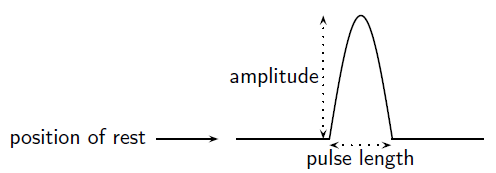
\includegraphics[width=300px]{col11305.imgs/m38801_PG10C4_002.png} % m38801;PG10C4\_002.png;;;6.0;8.5;
        
      \vspace{2pt}
    \vspace{\rubberspace}\par \begin{cnxcaption}
	  \small \textbf{Figure 6.2: }Example of a transverse pulse
	\end{cnxcaption}
      
    \vspace{.1in}
    \rule[.1in]{\figurerulewidth}{.005in} \\
        
    \end{center}

 \end{figure}   

    \addtocounter{footnote}{-0}
    
\label{m38801*eip-400}The position of rest is the position the medium would be in if it were undisturbed. This is also called the equilibrium position. Sometimes people will use rest and sometimes equilibrium but they will also use to the two in the same discussion to mean the same thing.\par \label{m38801*secfhsst!!!underscore!!!id87}
            \subsubsection{  Investigation : Pulse Length and Amplitude }
            \nopagebreak
            
        \label{m38801*id312993}The graphs below show the positions of a pulse at different times.\par 
        \label{m38801*id312998}
          
    \setcounter{subfigure}{0}


	\begin{figure}[H] % horizontal\label{m38801*id313002}
    \begin{center}
    \label{m38801*id313002!!!underscore!!!media}\label{m38801*id313002!!!underscore!!!printimage}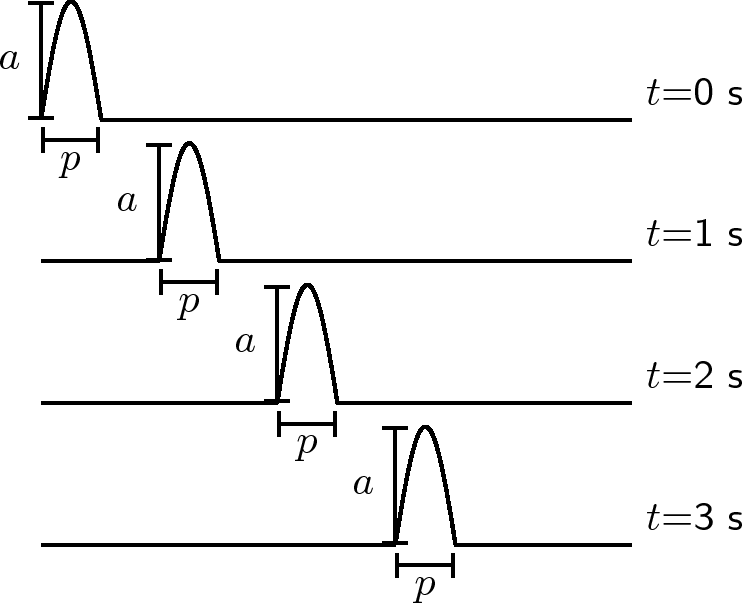
\includegraphics[width=300px]{col11305.imgs/m38801_PG10C4_003.png} % m38801;PG10C4\_003.png;;;6.0;8.5;
        
      \vspace{2pt}
    \vspace{.1in}
    
    \end{center}

 \end{figure}   

    \addtocounter{footnote}{-0}
    
        \par 
        \label{m38801*id313008}Use your ruler to measure the lengths of \begin{math}a\end{math} and \begin{math}p\end{math}. Fill your answers in the table.\par 
        
    % \textbf{m38801*id313027}\par
    
    % how many colspecs?  3
          % name: cnx:colspec
            % colnum: 1
            % colwidth: 10*
            % latex-name: columna
            % colname: 
            % align/tgroup-align/default: //left
            % -------------------------
            % name: cnx:colspec
            % colnum: 2
            % colwidth: 10*
            % latex-name: columnb
            % colname: 
            % align/tgroup-align/default: //left
            % -------------------------
            % name: cnx:colspec
            % colnum: 3
            % colwidth: 10*
            % latex-name: columnc
            % colname: 
            % align/tgroup-align/default: //left
            % -------------------------
      
    
    \setlength\mytablespace{6\tabcolsep}
    \addtolength\mytablespace{4\arrayrulewidth}
    \setlength\mytablewidth{\linewidth}
        
    
    \setlength\mytableroom{\mytablewidth}
    \addtolength\mytableroom{-\mytablespace}
    
    \setlength\myfixedwidth{0pt}
    \setlength\mystarwidth{\mytableroom}
        \addtolength\mystarwidth{-\myfixedwidth}
        \divide\mystarwidth 30
        
    
      % ----- Begin capturing width of table in LR mode woof
      \settowidth{\mytableboxwidth}{\begin{tabular}[t]{|l|l|l|}\hline
    % count in rowspan-info-nodeset: 3
    % align/colidx: left,1
    
    % rowcount: '0' | start: 'false' | colidx: '1'
    
        % Formatting a regular cell and recurring on the next sibling
        Time &
      % align/colidx: left,2
    
    % rowcount: '0' | start: 'false' | colidx: '2'
    
        % Formatting a regular cell and recurring on the next sibling
        
                  \begin{math}a\end{math}
                 &
      % align/colidx: left,3
    
    % rowcount: '0' | start: 'false' | colidx: '3'
    
        % Formatting a regular cell and recurring on the next sibling
        
                  \begin{math}p\end{math}
                % make-rowspan-placeholders
    % rowspan info: col1 '0' | 'false' | '' || col2 '0' | 'false' | '' || col3 '0' | 'false' | ''
     \tabularnewline\cline{1-1}\cline{2-2}\cline{3-3}
      %--------------------------------------------------------------------
    % align/colidx: left,1
    
    % rowcount: '0' | start: 'false' | colidx: '1'
    
        % Formatting a regular cell and recurring on the next sibling
        \begin{math}t=0\end{math}~s &
      % align/colidx: left,2
    
    % rowcount: '0' | start: 'false' | colidx: '2'
    
        % Formatting a regular cell and recurring on the next sibling
         &
      % align/colidx: left,3
    
    % rowcount: '0' | start: 'false' | colidx: '3'
    
        % Formatting a regular cell and recurring on the next sibling
        % make-rowspan-placeholders
    % rowspan info: col1 '0' | 'false' | '' || col2 '0' | 'false' | '' || col3 '0' | 'false' | ''
     \tabularnewline\cline{1-1}\cline{2-2}\cline{3-3}
      %--------------------------------------------------------------------
    % align/colidx: left,1
    
    % rowcount: '0' | start: 'false' | colidx: '1'
    
        % Formatting a regular cell and recurring on the next sibling
        \begin{math}t=1\end{math}~s &
      % align/colidx: left,2
    
    % rowcount: '0' | start: 'false' | colidx: '2'
    
        % Formatting a regular cell and recurring on the next sibling
         &
      % align/colidx: left,3
    
    % rowcount: '0' | start: 'false' | colidx: '3'
    
        % Formatting a regular cell and recurring on the next sibling
        % make-rowspan-placeholders
    % rowspan info: col1 '0' | 'false' | '' || col2 '0' | 'false' | '' || col3 '0' | 'false' | ''
     \tabularnewline\cline{1-1}\cline{2-2}\cline{3-3}
      %--------------------------------------------------------------------
    % align/colidx: left,1
    
    % rowcount: '0' | start: 'false' | colidx: '1'
    
        % Formatting a regular cell and recurring on the next sibling
        \begin{math}t=2\end{math}~s &
      % align/colidx: left,2
    
    % rowcount: '0' | start: 'false' | colidx: '2'
    
        % Formatting a regular cell and recurring on the next sibling
         &
      % align/colidx: left,3
    
    % rowcount: '0' | start: 'false' | colidx: '3'
    
        % Formatting a regular cell and recurring on the next sibling
        % make-rowspan-placeholders
    % rowspan info: col1 '0' | 'false' | '' || col2 '0' | 'false' | '' || col3 '0' | 'false' | ''
     \tabularnewline\cline{1-1}\cline{2-2}\cline{3-3}
      %--------------------------------------------------------------------
    % align/colidx: left,1
    
    % rowcount: '0' | start: 'false' | colidx: '1'
    
        % Formatting a regular cell and recurring on the next sibling
        \begin{math}t=3\end{math}~s &
      % align/colidx: left,2
    
    % rowcount: '0' | start: 'false' | colidx: '2'
    
        % Formatting a regular cell and recurring on the next sibling
         &
      % align/colidx: left,3
    
    % rowcount: '0' | start: 'false' | colidx: '3'
    
        % Formatting a regular cell and recurring on the next sibling
        % make-rowspan-placeholders
    % rowspan info: col1 '0' | 'false' | '' || col2 '0' | 'false' | '' || col3 '0' | 'false' | ''
     \tabularnewline\cline{1-1}\cline{2-2}\cline{3-3}
      %--------------------------------------------------------------------
    \end{tabular}} % end mytableboxwidth set
      \addtocounter{footnote}{-0}
      
      % ----- End capturing width of table in LR mode
    
        % ----- LR or paragraph mode: must test
        % ----- Begin capturing height of table
        \settoheight{\mytableboxheight}{\begin{tabular}[t]{|l|l|l|}\hline
    % count in rowspan-info-nodeset: 3
    % align/colidx: left,1
    
    % rowcount: '0' | start: 'false' | colidx: '1'
    
        % Formatting a regular cell and recurring on the next sibling
        Time &
      % align/colidx: left,2
    
    % rowcount: '0' | start: 'false' | colidx: '2'
    
        % Formatting a regular cell and recurring on the next sibling
        
                  \begin{math}a\end{math}
                 &
      % align/colidx: left,3
    
    % rowcount: '0' | start: 'false' | colidx: '3'
    
        % Formatting a regular cell and recurring on the next sibling
        
                  \begin{math}p\end{math}
                % make-rowspan-placeholders
    % rowspan info: col1 '0' | 'false' | '' || col2 '0' | 'false' | '' || col3 '0' | 'false' | ''
     \tabularnewline\cline{1-1}\cline{2-2}\cline{3-3}
      %--------------------------------------------------------------------
    % align/colidx: left,1
    
    % rowcount: '0' | start: 'false' | colidx: '1'
    
        % Formatting a regular cell and recurring on the next sibling
        \begin{math}t=0\end{math}~s &
      % align/colidx: left,2
    
    % rowcount: '0' | start: 'false' | colidx: '2'
    
        % Formatting a regular cell and recurring on the next sibling
         &
      % align/colidx: left,3
    
    % rowcount: '0' | start: 'false' | colidx: '3'
    
        % Formatting a regular cell and recurring on the next sibling
        % make-rowspan-placeholders
    % rowspan info: col1 '0' | 'false' | '' || col2 '0' | 'false' | '' || col3 '0' | 'false' | ''
     \tabularnewline\cline{1-1}\cline{2-2}\cline{3-3}
      %--------------------------------------------------------------------
    % align/colidx: left,1
    
    % rowcount: '0' | start: 'false' | colidx: '1'
    
        % Formatting a regular cell and recurring on the next sibling
        \begin{math}t=1\end{math}~s &
      % align/colidx: left,2
    
    % rowcount: '0' | start: 'false' | colidx: '2'
    
        % Formatting a regular cell and recurring on the next sibling
         &
      % align/colidx: left,3
    
    % rowcount: '0' | start: 'false' | colidx: '3'
    
        % Formatting a regular cell and recurring on the next sibling
        % make-rowspan-placeholders
    % rowspan info: col1 '0' | 'false' | '' || col2 '0' | 'false' | '' || col3 '0' | 'false' | ''
     \tabularnewline\cline{1-1}\cline{2-2}\cline{3-3}
      %--------------------------------------------------------------------
    % align/colidx: left,1
    
    % rowcount: '0' | start: 'false' | colidx: '1'
    
        % Formatting a regular cell and recurring on the next sibling
        \begin{math}t=2\end{math}~s &
      % align/colidx: left,2
    
    % rowcount: '0' | start: 'false' | colidx: '2'
    
        % Formatting a regular cell and recurring on the next sibling
         &
      % align/colidx: left,3
    
    % rowcount: '0' | start: 'false' | colidx: '3'
    
        % Formatting a regular cell and recurring on the next sibling
        % make-rowspan-placeholders
    % rowspan info: col1 '0' | 'false' | '' || col2 '0' | 'false' | '' || col3 '0' | 'false' | ''
     \tabularnewline\cline{1-1}\cline{2-2}\cline{3-3}
      %--------------------------------------------------------------------
    % align/colidx: left,1
    
    % rowcount: '0' | start: 'false' | colidx: '1'
    
        % Formatting a regular cell and recurring on the next sibling
        \begin{math}t=3\end{math}~s &
      % align/colidx: left,2
    
    % rowcount: '0' | start: 'false' | colidx: '2'
    
        % Formatting a regular cell and recurring on the next sibling
         &
      % align/colidx: left,3
    
    % rowcount: '0' | start: 'false' | colidx: '3'
    
        % Formatting a regular cell and recurring on the next sibling
        % make-rowspan-placeholders
    % rowspan info: col1 '0' | 'false' | '' || col2 '0' | 'false' | '' || col3 '0' | 'false' | ''
     \tabularnewline\cline{1-1}\cline{2-2}\cline{3-3}
      %--------------------------------------------------------------------
    \end{tabular}} % end mytableboxheight set
        \settodepth{\mytableboxdepth}{\begin{tabular}[t]{|l|l|l|}\hline
    % count in rowspan-info-nodeset: 3
    % align/colidx: left,1
    
    % rowcount: '0' | start: 'false' | colidx: '1'
    
        % Formatting a regular cell and recurring on the next sibling
        Time &
      % align/colidx: left,2
    
    % rowcount: '0' | start: 'false' | colidx: '2'
    
        % Formatting a regular cell and recurring on the next sibling
        
                  \begin{math}a\end{math}
                 &
      % align/colidx: left,3
    
    % rowcount: '0' | start: 'false' | colidx: '3'
    
        % Formatting a regular cell and recurring on the next sibling
        
                  \begin{math}p\end{math}
                % make-rowspan-placeholders
    % rowspan info: col1 '0' | 'false' | '' || col2 '0' | 'false' | '' || col3 '0' | 'false' | ''
     \tabularnewline\cline{1-1}\cline{2-2}\cline{3-3}
      %--------------------------------------------------------------------
    % align/colidx: left,1
    
    % rowcount: '0' | start: 'false' | colidx: '1'
    
        % Formatting a regular cell and recurring on the next sibling
        \begin{math}t=0\end{math}~s &
      % align/colidx: left,2
    
    % rowcount: '0' | start: 'false' | colidx: '2'
    
        % Formatting a regular cell and recurring on the next sibling
         &
      % align/colidx: left,3
    
    % rowcount: '0' | start: 'false' | colidx: '3'
    
        % Formatting a regular cell and recurring on the next sibling
        % make-rowspan-placeholders
    % rowspan info: col1 '0' | 'false' | '' || col2 '0' | 'false' | '' || col3 '0' | 'false' | ''
     \tabularnewline\cline{1-1}\cline{2-2}\cline{3-3}
      %--------------------------------------------------------------------
    % align/colidx: left,1
    
    % rowcount: '0' | start: 'false' | colidx: '1'
    
        % Formatting a regular cell and recurring on the next sibling
        \begin{math}t=1\end{math}~s &
      % align/colidx: left,2
    
    % rowcount: '0' | start: 'false' | colidx: '2'
    
        % Formatting a regular cell and recurring on the next sibling
         &
      % align/colidx: left,3
    
    % rowcount: '0' | start: 'false' | colidx: '3'
    
        % Formatting a regular cell and recurring on the next sibling
        % make-rowspan-placeholders
    % rowspan info: col1 '0' | 'false' | '' || col2 '0' | 'false' | '' || col3 '0' | 'false' | ''
     \tabularnewline\cline{1-1}\cline{2-2}\cline{3-3}
      %--------------------------------------------------------------------
    % align/colidx: left,1
    
    % rowcount: '0' | start: 'false' | colidx: '1'
    
        % Formatting a regular cell and recurring on the next sibling
        \begin{math}t=2\end{math}~s &
      % align/colidx: left,2
    
    % rowcount: '0' | start: 'false' | colidx: '2'
    
        % Formatting a regular cell and recurring on the next sibling
         &
      % align/colidx: left,3
    
    % rowcount: '0' | start: 'false' | colidx: '3'
    
        % Formatting a regular cell and recurring on the next sibling
        % make-rowspan-placeholders
    % rowspan info: col1 '0' | 'false' | '' || col2 '0' | 'false' | '' || col3 '0' | 'false' | ''
     \tabularnewline\cline{1-1}\cline{2-2}\cline{3-3}
      %--------------------------------------------------------------------
    % align/colidx: left,1
    
    % rowcount: '0' | start: 'false' | colidx: '1'
    
        % Formatting a regular cell and recurring on the next sibling
        \begin{math}t=3\end{math}~s &
      % align/colidx: left,2
    
    % rowcount: '0' | start: 'false' | colidx: '2'
    
        % Formatting a regular cell and recurring on the next sibling
         &
      % align/colidx: left,3
    
    % rowcount: '0' | start: 'false' | colidx: '3'
    
        % Formatting a regular cell and recurring on the next sibling
        % make-rowspan-placeholders
    % rowspan info: col1 '0' | 'false' | '' || col2 '0' | 'false' | '' || col3 '0' | 'false' | ''
     \tabularnewline\cline{1-1}\cline{2-2}\cline{3-3}
      %--------------------------------------------------------------------
    \end{tabular}} % end mytableboxdepth set
        \addtolength{\mytableboxheight}{\mytableboxdepth}
        % ----- End capturing height of table
        \addtocounter{footnote}{-0}
        
        \ifthenelse{\mytableboxwidth<\textwidth}{% the table fits in LR mode
          \addtolength{\mytableboxwidth}{-\mytablespace}
          \typeout{textheight: \the\textheight}
          \typeout{mytableboxheight: \the\mytableboxheight}
          \typeout{textwidth: \the\textwidth}
          \typeout{mytableboxwidth: \the\mytableboxwidth}
          \ifthenelse{\mytableboxheight<\textheight}{%
        
    % \begin{table}[H]
    % \\ '' '0'
    
        \begin{center}
      
      \label{m38801*id313027}
      
    \noindent
    \begin{tabular}[t]{|l|l|l|}\hline
    % count in rowspan-info-nodeset: 3
    % align/colidx: left,1
    
    % rowcount: '0' | start: 'false' | colidx: '1'
    
        % Formatting a regular cell and recurring on the next sibling
        Time &
      % align/colidx: left,2
    
    % rowcount: '0' | start: 'false' | colidx: '2'
    
        % Formatting a regular cell and recurring on the next sibling
        
                  \begin{math}a\end{math}
                 &
      % align/colidx: left,3
    
    % rowcount: '0' | start: 'false' | colidx: '3'
    
        % Formatting a regular cell and recurring on the next sibling
        
                  \begin{math}p\end{math}
                % make-rowspan-placeholders
    % rowspan info: col1 '0' | 'false' | '' || col2 '0' | 'false' | '' || col3 '0' | 'false' | ''
     \tabularnewline\cline{1-1}\cline{2-2}\cline{3-3}
      %--------------------------------------------------------------------
    % align/colidx: left,1
    
    % rowcount: '0' | start: 'false' | colidx: '1'
    
        % Formatting a regular cell and recurring on the next sibling
        \begin{math}t=0\end{math}~s &
      % align/colidx: left,2
    
    % rowcount: '0' | start: 'false' | colidx: '2'
    
        % Formatting a regular cell and recurring on the next sibling
         &
      % align/colidx: left,3
    
    % rowcount: '0' | start: 'false' | colidx: '3'
    
        % Formatting a regular cell and recurring on the next sibling
        % make-rowspan-placeholders
    % rowspan info: col1 '0' | 'false' | '' || col2 '0' | 'false' | '' || col3 '0' | 'false' | ''
     \tabularnewline\cline{1-1}\cline{2-2}\cline{3-3}
      %--------------------------------------------------------------------
    % align/colidx: left,1
    
    % rowcount: '0' | start: 'false' | colidx: '1'
    
        % Formatting a regular cell and recurring on the next sibling
        \begin{math}t=1\end{math}~s &
      % align/colidx: left,2
    
    % rowcount: '0' | start: 'false' | colidx: '2'
    
        % Formatting a regular cell and recurring on the next sibling
         &
      % align/colidx: left,3
    
    % rowcount: '0' | start: 'false' | colidx: '3'
    
        % Formatting a regular cell and recurring on the next sibling
        % make-rowspan-placeholders
    % rowspan info: col1 '0' | 'false' | '' || col2 '0' | 'false' | '' || col3 '0' | 'false' | ''
     \tabularnewline\cline{1-1}\cline{2-2}\cline{3-3}
      %--------------------------------------------------------------------
    % align/colidx: left,1
    
    % rowcount: '0' | start: 'false' | colidx: '1'
    
        % Formatting a regular cell and recurring on the next sibling
        \begin{math}t=2\end{math}~s &
      % align/colidx: left,2
    
    % rowcount: '0' | start: 'false' | colidx: '2'
    
        % Formatting a regular cell and recurring on the next sibling
         &
      % align/colidx: left,3
    
    % rowcount: '0' | start: 'false' | colidx: '3'
    
        % Formatting a regular cell and recurring on the next sibling
        % make-rowspan-placeholders
    % rowspan info: col1 '0' | 'false' | '' || col2 '0' | 'false' | '' || col3 '0' | 'false' | ''
     \tabularnewline\cline{1-1}\cline{2-2}\cline{3-3}
      %--------------------------------------------------------------------
    % align/colidx: left,1
    
    % rowcount: '0' | start: 'false' | colidx: '1'
    
        % Formatting a regular cell and recurring on the next sibling
        \begin{math}t=3\end{math}~s &
      % align/colidx: left,2
    
    % rowcount: '0' | start: 'false' | colidx: '2'
    
        % Formatting a regular cell and recurring on the next sibling
         &
      % align/colidx: left,3
    
    % rowcount: '0' | start: 'false' | colidx: '3'
    
        % Formatting a regular cell and recurring on the next sibling
        % make-rowspan-placeholders
    % rowspan info: col1 '0' | 'false' | '' || col2 '0' | 'false' | '' || col3 '0' | 'false' | ''
     \tabularnewline\cline{1-1}\cline{2-2}\cline{3-3}
      %--------------------------------------------------------------------
    \end{tabular}
      \end{center}
    \begin{center}{\small\bfseries Table 6.1}\end{center}
    %\end{table}
    
    \addtocounter{footnote}{-0}
    
          }{ % else
        
    % \begin{table}[H]
    % \\ '' '0'
    
        \begin{center}
      
      \label{m38801*id313027}
      
    \noindent
    \tabletail{%
        \hline
        \multicolumn{3}{|p{\mytableboxwidth}|}{\raggedleft \small \sl continued on next page}\\
        \hline
      }
      \tablelasttail{}
      \begin{xtabular}[t]{|l|l|l|}\hline
    % count in rowspan-info-nodeset: 3
    % align/colidx: left,1
    
    % rowcount: '0' | start: 'false' | colidx: '1'
    
        % Formatting a regular cell and recurring on the next sibling
        Time &
      % align/colidx: left,2
    
    % rowcount: '0' | start: 'false' | colidx: '2'
    
        % Formatting a regular cell and recurring on the next sibling
        
                  \begin{math}a\end{math}
                 &
      % align/colidx: left,3
    
    % rowcount: '0' | start: 'false' | colidx: '3'
    
        % Formatting a regular cell and recurring on the next sibling
        
                  \begin{math}p\end{math}
                % make-rowspan-placeholders
    % rowspan info: col1 '0' | 'false' | '' || col2 '0' | 'false' | '' || col3 '0' | 'false' | ''
     \tabularnewline\cline{1-1}\cline{2-2}\cline{3-3}
      %--------------------------------------------------------------------
    % align/colidx: left,1
    
    % rowcount: '0' | start: 'false' | colidx: '1'
    
        % Formatting a regular cell and recurring on the next sibling
        \begin{math}t=0\end{math}~s &
      % align/colidx: left,2
    
    % rowcount: '0' | start: 'false' | colidx: '2'
    
        % Formatting a regular cell and recurring on the next sibling
         &
      % align/colidx: left,3
    
    % rowcount: '0' | start: 'false' | colidx: '3'
    
        % Formatting a regular cell and recurring on the next sibling
        % make-rowspan-placeholders
    % rowspan info: col1 '0' | 'false' | '' || col2 '0' | 'false' | '' || col3 '0' | 'false' | ''
     \tabularnewline\cline{1-1}\cline{2-2}\cline{3-3}
      %--------------------------------------------------------------------
    % align/colidx: left,1
    
    % rowcount: '0' | start: 'false' | colidx: '1'
    
        % Formatting a regular cell and recurring on the next sibling
        \begin{math}t=1\end{math}~s &
      % align/colidx: left,2
    
    % rowcount: '0' | start: 'false' | colidx: '2'
    
        % Formatting a regular cell and recurring on the next sibling
         &
      % align/colidx: left,3
    
    % rowcount: '0' | start: 'false' | colidx: '3'
    
        % Formatting a regular cell and recurring on the next sibling
        % make-rowspan-placeholders
    % rowspan info: col1 '0' | 'false' | '' || col2 '0' | 'false' | '' || col3 '0' | 'false' | ''
     \tabularnewline\cline{1-1}\cline{2-2}\cline{3-3}
      %--------------------------------------------------------------------
    % align/colidx: left,1
    
    % rowcount: '0' | start: 'false' | colidx: '1'
    
        % Formatting a regular cell and recurring on the next sibling
        \begin{math}t=2\end{math}~s &
      % align/colidx: left,2
    
    % rowcount: '0' | start: 'false' | colidx: '2'
    
        % Formatting a regular cell and recurring on the next sibling
         &
      % align/colidx: left,3
    
    % rowcount: '0' | start: 'false' | colidx: '3'
    
        % Formatting a regular cell and recurring on the next sibling
        % make-rowspan-placeholders
    % rowspan info: col1 '0' | 'false' | '' || col2 '0' | 'false' | '' || col3 '0' | 'false' | ''
     \tabularnewline\cline{1-1}\cline{2-2}\cline{3-3}
      %--------------------------------------------------------------------
    % align/colidx: left,1
    
    % rowcount: '0' | start: 'false' | colidx: '1'
    
        % Formatting a regular cell and recurring on the next sibling
        \begin{math}t=3\end{math}~s &
      % align/colidx: left,2
    
    % rowcount: '0' | start: 'false' | colidx: '2'
    
        % Formatting a regular cell and recurring on the next sibling
         &
      % align/colidx: left,3
    
    % rowcount: '0' | start: 'false' | colidx: '3'
    
        % Formatting a regular cell and recurring on the next sibling
        % make-rowspan-placeholders
    % rowspan info: col1 '0' | 'false' | '' || col2 '0' | 'false' | '' || col3 '0' | 'false' | ''
     \tabularnewline\cline{1-1}\cline{2-2}\cline{3-3}
      %--------------------------------------------------------------------
    \end{xtabular}
      \end{center}
    \begin{center}{\small\bfseries Table 6.1}\end{center}
    %\end{table}
    
    \addtocounter{footnote}{-0}
    
          } % 
        }{% else
        % typeset the table in paragraph mode
        % ----- Begin capturing height of table
        \settoheight{\mytableboxheight}{\begin{tabular*}{\mytablewidth}[t]{|p{10\mystarwidth}|p{10\mystarwidth}|p{10\mystarwidth}|}\hline
    % count in rowspan-info-nodeset: 3
    % align/colidx: left,1
    
    % rowcount: '0' | start: 'false' | colidx: '1'
    
        % Formatting a regular cell and recurring on the next sibling
        Time &
      % align/colidx: left,2
    
    % rowcount: '0' | start: 'false' | colidx: '2'
    
        % Formatting a regular cell and recurring on the next sibling
        
                  \begin{math}a\end{math}
                 &
      % align/colidx: left,3
    
    % rowcount: '0' | start: 'false' | colidx: '3'
    
        % Formatting a regular cell and recurring on the next sibling
        
                  \begin{math}p\end{math}
                % make-rowspan-placeholders
    % rowspan info: col1 '0' | 'false' | '' || col2 '0' | 'false' | '' || col3 '0' | 'false' | ''
     \tabularnewline\cline{1-1}\cline{2-2}\cline{3-3}
      %--------------------------------------------------------------------
    % align/colidx: left,1
    
    % rowcount: '0' | start: 'false' | colidx: '1'
    
        % Formatting a regular cell and recurring on the next sibling
        \begin{math}t=0\end{math}~s &
      % align/colidx: left,2
    
    % rowcount: '0' | start: 'false' | colidx: '2'
    
        % Formatting a regular cell and recurring on the next sibling
         &
      % align/colidx: left,3
    
    % rowcount: '0' | start: 'false' | colidx: '3'
    
        % Formatting a regular cell and recurring on the next sibling
        % make-rowspan-placeholders
    % rowspan info: col1 '0' | 'false' | '' || col2 '0' | 'false' | '' || col3 '0' | 'false' | ''
     \tabularnewline\cline{1-1}\cline{2-2}\cline{3-3}
      %--------------------------------------------------------------------
    % align/colidx: left,1
    
    % rowcount: '0' | start: 'false' | colidx: '1'
    
        % Formatting a regular cell and recurring on the next sibling
        \begin{math}t=1\end{math}~s &
      % align/colidx: left,2
    
    % rowcount: '0' | start: 'false' | colidx: '2'
    
        % Formatting a regular cell and recurring on the next sibling
         &
      % align/colidx: left,3
    
    % rowcount: '0' | start: 'false' | colidx: '3'
    
        % Formatting a regular cell and recurring on the next sibling
        % make-rowspan-placeholders
    % rowspan info: col1 '0' | 'false' | '' || col2 '0' | 'false' | '' || col3 '0' | 'false' | ''
     \tabularnewline\cline{1-1}\cline{2-2}\cline{3-3}
      %--------------------------------------------------------------------
    % align/colidx: left,1
    
    % rowcount: '0' | start: 'false' | colidx: '1'
    
        % Formatting a regular cell and recurring on the next sibling
        \begin{math}t=2\end{math}~s &
      % align/colidx: left,2
    
    % rowcount: '0' | start: 'false' | colidx: '2'
    
        % Formatting a regular cell and recurring on the next sibling
         &
      % align/colidx: left,3
    
    % rowcount: '0' | start: 'false' | colidx: '3'
    
        % Formatting a regular cell and recurring on the next sibling
        % make-rowspan-placeholders
    % rowspan info: col1 '0' | 'false' | '' || col2 '0' | 'false' | '' || col3 '0' | 'false' | ''
     \tabularnewline\cline{1-1}\cline{2-2}\cline{3-3}
      %--------------------------------------------------------------------
    % align/colidx: left,1
    
    % rowcount: '0' | start: 'false' | colidx: '1'
    
        % Formatting a regular cell and recurring on the next sibling
        \begin{math}t=3\end{math}~s &
      % align/colidx: left,2
    
    % rowcount: '0' | start: 'false' | colidx: '2'
    
        % Formatting a regular cell and recurring on the next sibling
         &
      % align/colidx: left,3
    
    % rowcount: '0' | start: 'false' | colidx: '3'
    
        % Formatting a regular cell and recurring on the next sibling
        % make-rowspan-placeholders
    % rowspan info: col1 '0' | 'false' | '' || col2 '0' | 'false' | '' || col3 '0' | 'false' | ''
     \tabularnewline\cline{1-1}\cline{2-2}\cline{3-3}
      %--------------------------------------------------------------------
    \end{tabular*}} % end mytableboxheight set
        \settodepth{\mytableboxdepth}{\begin{tabular*}{\mytablewidth}[t]{|p{10\mystarwidth}|p{10\mystarwidth}|p{10\mystarwidth}|}\hline
    % count in rowspan-info-nodeset: 3
    % align/colidx: left,1
    
    % rowcount: '0' | start: 'false' | colidx: '1'
    
        % Formatting a regular cell and recurring on the next sibling
        Time &
      % align/colidx: left,2
    
    % rowcount: '0' | start: 'false' | colidx: '2'
    
        % Formatting a regular cell and recurring on the next sibling
        
                  \begin{math}a\end{math}
                 &
      % align/colidx: left,3
    
    % rowcount: '0' | start: 'false' | colidx: '3'
    
        % Formatting a regular cell and recurring on the next sibling
        
                  \begin{math}p\end{math}
                % make-rowspan-placeholders
    % rowspan info: col1 '0' | 'false' | '' || col2 '0' | 'false' | '' || col3 '0' | 'false' | ''
     \tabularnewline\cline{1-1}\cline{2-2}\cline{3-3}
      %--------------------------------------------------------------------
    % align/colidx: left,1
    
    % rowcount: '0' | start: 'false' | colidx: '1'
    
        % Formatting a regular cell and recurring on the next sibling
        \begin{math}t=0\end{math}~s &
      % align/colidx: left,2
    
    % rowcount: '0' | start: 'false' | colidx: '2'
    
        % Formatting a regular cell and recurring on the next sibling
         &
      % align/colidx: left,3
    
    % rowcount: '0' | start: 'false' | colidx: '3'
    
        % Formatting a regular cell and recurring on the next sibling
        % make-rowspan-placeholders
    % rowspan info: col1 '0' | 'false' | '' || col2 '0' | 'false' | '' || col3 '0' | 'false' | ''
     \tabularnewline\cline{1-1}\cline{2-2}\cline{3-3}
      %--------------------------------------------------------------------
    % align/colidx: left,1
    
    % rowcount: '0' | start: 'false' | colidx: '1'
    
        % Formatting a regular cell and recurring on the next sibling
        \begin{math}t=1\end{math}~s &
      % align/colidx: left,2
    
    % rowcount: '0' | start: 'false' | colidx: '2'
    
        % Formatting a regular cell and recurring on the next sibling
         &
      % align/colidx: left,3
    
    % rowcount: '0' | start: 'false' | colidx: '3'
    
        % Formatting a regular cell and recurring on the next sibling
        % make-rowspan-placeholders
    % rowspan info: col1 '0' | 'false' | '' || col2 '0' | 'false' | '' || col3 '0' | 'false' | ''
     \tabularnewline\cline{1-1}\cline{2-2}\cline{3-3}
      %--------------------------------------------------------------------
    % align/colidx: left,1
    
    % rowcount: '0' | start: 'false' | colidx: '1'
    
        % Formatting a regular cell and recurring on the next sibling
        \begin{math}t=2\end{math}~s &
      % align/colidx: left,2
    
    % rowcount: '0' | start: 'false' | colidx: '2'
    
        % Formatting a regular cell and recurring on the next sibling
         &
      % align/colidx: left,3
    
    % rowcount: '0' | start: 'false' | colidx: '3'
    
        % Formatting a regular cell and recurring on the next sibling
        % make-rowspan-placeholders
    % rowspan info: col1 '0' | 'false' | '' || col2 '0' | 'false' | '' || col3 '0' | 'false' | ''
     \tabularnewline\cline{1-1}\cline{2-2}\cline{3-3}
      %--------------------------------------------------------------------
    % align/colidx: left,1
    
    % rowcount: '0' | start: 'false' | colidx: '1'
    
        % Formatting a regular cell and recurring on the next sibling
        \begin{math}t=3\end{math}~s &
      % align/colidx: left,2
    
    % rowcount: '0' | start: 'false' | colidx: '2'
    
        % Formatting a regular cell and recurring on the next sibling
         &
      % align/colidx: left,3
    
    % rowcount: '0' | start: 'false' | colidx: '3'
    
        % Formatting a regular cell and recurring on the next sibling
        % make-rowspan-placeholders
    % rowspan info: col1 '0' | 'false' | '' || col2 '0' | 'false' | '' || col3 '0' | 'false' | ''
     \tabularnewline\cline{1-1}\cline{2-2}\cline{3-3}
      %--------------------------------------------------------------------
    \end{tabular*}} % end mytableboxdepth set
        \addtolength{\mytableboxheight}{\mytableboxdepth}
        % ----- End capturing height of table
        \typeout{textheight: \the\textheight}
        \typeout{mytableboxheight: \the\mytableboxheight}
        \typeout{table too wide, outputting in para mode}
        
    % \begin{table}[H]
    % \\ '' '0'
    
        \begin{center}
      
      \label{m38801*id313027}
      
    \noindent
    \tabletail{%
        \hline
        \multicolumn{3}{|p{\mytableroom}|}{\raggedleft \small \sl continued on next page}\\
        \hline
      }
      \tablelasttail{}
      \begin{xtabular*}{\mytablewidth}[t]{|p{10\mystarwidth}|p{10\mystarwidth}|p{10\mystarwidth}|}\hline
    % count in rowspan-info-nodeset: 3
    % align/colidx: left,1
    
    % rowcount: '0' | start: 'false' | colidx: '1'
    
        % Formatting a regular cell and recurring on the next sibling
        Time &
      % align/colidx: left,2
    
    % rowcount: '0' | start: 'false' | colidx: '2'
    
        % Formatting a regular cell and recurring on the next sibling
        
                  \begin{math}a\end{math}
                 &
      % align/colidx: left,3
    
    % rowcount: '0' | start: 'false' | colidx: '3'
    
        % Formatting a regular cell and recurring on the next sibling
        
                  \begin{math}p\end{math}
                % make-rowspan-placeholders
    % rowspan info: col1 '0' | 'false' | '' || col2 '0' | 'false' | '' || col3 '0' | 'false' | ''
     \tabularnewline\cline{1-1}\cline{2-2}\cline{3-3}
      %--------------------------------------------------------------------
    % align/colidx: left,1
    
    % rowcount: '0' | start: 'false' | colidx: '1'
    
        % Formatting a regular cell and recurring on the next sibling
        \begin{math}t=0\end{math}~s &
      % align/colidx: left,2
    
    % rowcount: '0' | start: 'false' | colidx: '2'
    
        % Formatting a regular cell and recurring on the next sibling
         &
      % align/colidx: left,3
    
    % rowcount: '0' | start: 'false' | colidx: '3'
    
        % Formatting a regular cell and recurring on the next sibling
        % make-rowspan-placeholders
    % rowspan info: col1 '0' | 'false' | '' || col2 '0' | 'false' | '' || col3 '0' | 'false' | ''
     \tabularnewline\cline{1-1}\cline{2-2}\cline{3-3}
      %--------------------------------------------------------------------
    % align/colidx: left,1
    
    % rowcount: '0' | start: 'false' | colidx: '1'
    
        % Formatting a regular cell and recurring on the next sibling
        \begin{math}t=1\end{math}~s &
      % align/colidx: left,2
    
    % rowcount: '0' | start: 'false' | colidx: '2'
    
        % Formatting a regular cell and recurring on the next sibling
         &
      % align/colidx: left,3
    
    % rowcount: '0' | start: 'false' | colidx: '3'
    
        % Formatting a regular cell and recurring on the next sibling
        % make-rowspan-placeholders
    % rowspan info: col1 '0' | 'false' | '' || col2 '0' | 'false' | '' || col3 '0' | 'false' | ''
     \tabularnewline\cline{1-1}\cline{2-2}\cline{3-3}
      %--------------------------------------------------------------------
    % align/colidx: left,1
    
    % rowcount: '0' | start: 'false' | colidx: '1'
    
        % Formatting a regular cell and recurring on the next sibling
        \begin{math}t=2\end{math}~s &
      % align/colidx: left,2
    
    % rowcount: '0' | start: 'false' | colidx: '2'
    
        % Formatting a regular cell and recurring on the next sibling
         &
      % align/colidx: left,3
    
    % rowcount: '0' | start: 'false' | colidx: '3'
    
        % Formatting a regular cell and recurring on the next sibling
        % make-rowspan-placeholders
    % rowspan info: col1 '0' | 'false' | '' || col2 '0' | 'false' | '' || col3 '0' | 'false' | ''
     \tabularnewline\cline{1-1}\cline{2-2}\cline{3-3}
      %--------------------------------------------------------------------
    % align/colidx: left,1
    
    % rowcount: '0' | start: 'false' | colidx: '1'
    
        % Formatting a regular cell and recurring on the next sibling
        \begin{math}t=3\end{math}~s &
      % align/colidx: left,2
    
    % rowcount: '0' | start: 'false' | colidx: '2'
    
        % Formatting a regular cell and recurring on the next sibling
         &
      % align/colidx: left,3
    
    % rowcount: '0' | start: 'false' | colidx: '3'
    
        % Formatting a regular cell and recurring on the next sibling
        % make-rowspan-placeholders
    % rowspan info: col1 '0' | 'false' | '' || col2 '0' | 'false' | '' || col3 '0' | 'false' | ''
     \tabularnewline\cline{1-1}\cline{2-2}\cline{3-3}
      %--------------------------------------------------------------------
    \end{xtabular*}
      \end{center}
    \begin{center}{\small\bfseries Table 6.1}\end{center}
    %\end{table}
    
    \addtocounter{footnote}{-0}
    
        }% ending lr/para test clause
      
    \par
  
        
        \label{m38801*id313222}What do you notice about the values of \begin{math}a\end{math} and \begin{math}p\end{math}?
 \par 

        \label{m38801*id313246}In the activity, we found that the values for how high the pulse (\begin{math}a\end{math}) is and how wide the pulse (\begin{math}p\end{math}) is the same at different times. \textsl{Pulse length} and \textsl{amplitude} are two important quantities of a pulse.\par 
      
      \label{m38801*uid3}
            \subsubsection{ Pulse Speed}
            \nopagebreak
            
        
\par
            \label{m38801*fhsst!!!underscore!!!id145}\begin{definition}
	  \begin{tabular*}{15 cm}{m{15 mm}m{}}
	\hspace*{-50pt}  
\includegraphics[width=0.5in]{col11305.imgs/psflag2.png}   & \Definition{   \label{id2435275}\textbf{ Pulse Speed }} { \label{m38801*meaningfhsst!!!underscore!!!id145}
        \label{m38801*id313292}Pulse speed is the distance a pulse travels per unit time. \par 
         } 
      \end{tabular*}
      \end{definition}

        \label{m38801*id313303}In Motion in one dimension\footnote{\raggedright{}"Motion in One Dimension - Grade 10 [CAPS]" <http://http://cnx.org/content/m37923/latest/>} we saw that speed was defined as the distance traveled per unit time. We can use the same definition of speed to calculate how fast a pulse travels. If the pulse travels a distance \begin{math}D\end{math} in a time \begin{math}t\end{math}, then the pulse speed \begin{math}v\end{math} is:\par 
        \label{m38801*uid4}\nopagebreak\noindent{}\settowidth{\mymathboxwidth}{\begin{equation}
    v=\frac{D}{t}\tag{6.1}
      \end{equation}
    }
    \typeout{Columnwidth = \the\columnwidth}\typeout{math as usual width = \the\mymathboxwidth}
    \ifthenelse{\lengthtest{\mymathboxwidth < \columnwidth}}{% if the math fits, do it again, for real
    \begin{equation}
    v=\frac{D}{t}\tag{6.1}
      \end{equation}
    }{% else, if it doesn't fit
    \setlength{\mymathboxwidth}{\columnwidth}
      \addtolength{\mymathboxwidth}{-48pt}
    \par\vspace{12pt}\noindent\begin{minipage}{\columnwidth}
    \parbox[t]{\mymathboxwidth}{\large\begin{math}
    v=\frac{D}{t}\end{math}}\hfill
    \parbox[t]{48pt}{\raggedleft 
    (6.1)}
    \end{minipage}\vspace{12pt}\par
    }% end of conditional for this bit of math
    \typeout{math as usual width = \the\mymathboxwidth}
    
        
\par
            \label{m38801*secfhsst!!!underscore!!!id161}\vspace{.5cm} 
      
      \noindent
      \hspace*{-30pt}
\includegraphics[width=0.5in]{col11305.imgs/pspencil2.png}   \raisebox{25mm}{   
      \begin{mdframed}[linewidth=4, leftmargin=40, rightmargin=40]  
      \begin{exercise}
    \noindent\textbf{Exercise 6.1:  Pulse Speed }
        \label{m38801*probfhsst!!!underscore!!!id162}
        \label{m38801*id313369}A pulse covers a distance of \begin{math}2\phantom{\rule{3pt}{0ex}}\mathrm{m}\end{math} in \begin{math}4\phantom{\rule{3pt}{0ex}}\mathrm{s}\end{math} on a heavy rope. Calculate the pulse speed. \par 
        \vspace{5pt}
        \label{m38801*solfhsst!!!underscore!!!id165}\noindent\textbf{Solution to Exercise } \label{m38801*listfhsst!!!underscore!!!id165}\begin{enumerate}[noitemsep, label=\textbf{Step} \textbf{\arabic*}. ] 
            \leftskip=20pt\rightskip=\leftskip\item  
        \label{m38801*id313393}We are given:\par 
        \label{m38801*id313396}\begin{itemize}[noitemsep]
            \leftskip=20pt\rightskip=\leftskip\label{m38801*uid5}\item the distance travelled by the pulse: \begin{math}D=2\phantom{\rule{2pt}{0ex}}\mathrm{m}\end{math}
\label{m38801*uid6}\item the time taken to travel \begin{math}2\phantom{\rule{2pt}{0ex}}\mathrm{m}\end{math}: \begin{math}t=4\phantom{\rule{2pt}{0ex}}\mathrm{s}\end{math}
\end{itemize}
        
        \label{m38801*id313439}We are required to calculate the speed of the pulse.\par 
        \item  
        \label{m38801*id313447}We can use:\par 
        \label{m38801*id313450}\nopagebreak\noindent{}\settowidth{\mymathboxwidth}{\begin{equation}
    v=\frac{D}{t}\tag{6.2}
      \end{equation}
    }
    \typeout{Columnwidth = \the\columnwidth}\typeout{math as usual width = \the\mymathboxwidth}
    \ifthenelse{\lengthtest{\mymathboxwidth < \columnwidth}}{% if the math fits, do it again, for real
    \begin{equation}
    v=\frac{D}{t}\tag{6.2}
      \end{equation}
    }{% else, if it doesn't fit
    \setlength{\mymathboxwidth}{\columnwidth}
      \addtolength{\mymathboxwidth}{-48pt}
    \par\vspace{12pt}\noindent\begin{minipage}{\columnwidth}
    \parbox[t]{\mymathboxwidth}{\large\begin{math}
    v=\frac{D}{t}\end{math}}\hfill
    \parbox[t]{48pt}{\raggedleft 
    (6.2)}
    \end{minipage}\vspace{12pt}\par
    }% end of conditional for this bit of math
    \typeout{math as usual width = \the\mymathboxwidth}
    
        
        \label{m38801*id313470}to calculate the speed of the pulse.\par 
        \item  
        \label{m38801*id313479}\nopagebreak\noindent{}\settowidth{\mymathboxwidth}{\begin{equation}
    \begin{array}{ccc}\hfill v& =& \frac{D}{t}\hfill \\ & =& \frac{2\phantom{\rule{0.166667em}{0ex}}\mathrm{m}}{4\phantom{\rule{0.166667em}{0ex}}\mathrm{s}}\hfill \\ & =& 0,5\phantom{\rule{0.166667em}{0ex}}\mathrm{m}\ensuremath{\cdot}{\mathrm{s}}^{-1}\hfill \end{array}\tag{6.3}
      \end{equation}
    }
    \typeout{Columnwidth = \the\columnwidth}\typeout{math as usual width = \the\mymathboxwidth}
    \ifthenelse{\lengthtest{\mymathboxwidth < \columnwidth}}{% if the math fits, do it again, for real
    \begin{equation}
    \begin{array}{ccc}\hfill v& =& \frac{D}{t}\hfill \\ & =& \frac{2\phantom{\rule{0.166667em}{0ex}}\mathrm{m}}{4\phantom{\rule{0.166667em}{0ex}}\mathrm{s}}\hfill \\ & =& 0,5\phantom{\rule{0.166667em}{0ex}}\mathrm{m}\ensuremath{\cdot}{\mathrm{s}}^{-1}\hfill \end{array}\tag{6.3}
      \end{equation}
    }{% else, if it doesn't fit
    \setlength{\mymathboxwidth}{\columnwidth}
      \addtolength{\mymathboxwidth}{-48pt}
    \par\vspace{12pt}\noindent\begin{minipage}{\columnwidth}
    \parbox[t]{\mymathboxwidth}{\large\begin{math}
    v=\frac{D}{t}=\frac{2\phantom{\rule{0.166667em}{0ex}}\mathrm{m}}{4\phantom{\rule{0.166667em}{0ex}}\mathrm{s}}=0,5\phantom{\rule{0.166667em}{0ex}}\mathrm{m}\ensuremath{\cdot}{\mathrm{s}}^{-1}\end{math}}\hfill
    \parbox[t]{48pt}{\raggedleft 
    (6.3)}
    \end{minipage}\vspace{12pt}\par
    }% end of conditional for this bit of math
    \typeout{math as usual width = \the\mymathboxwidth}
    
        
        \item  
        \label{m38801*id313763}The pulse speed is \begin{math}0,5\phantom{\rule{2pt}{0ex}}\mathrm{m}\ensuremath{\cdot}\mathrm{s}{}^{-1}\end{math}.
 \par 
        \end{enumerate}
         

    \end{exercise}
    \end{mdframed}
    }
    \noindent
  
\label{m38801*notfhsst!!!underscore!!!id259}
\begin{tabular}{cc}
	   \hspace*{-50pt}\raisebox{-8 mm}{ 
\includegraphics[width=0.5in]{col11305.imgs/pstip2.png}  }& 

	\begin{minipage}{0.85\textwidth}
	\begin{note}
      {tip: }The pulse speed depends on the properties of the medium and not on the amplitude or pulse length of the pulse.
	\end{note}
	\end{minipage}
	\end{tabular}
	\par
      
\label{m38801*secfhsst!!!underscore!!!id260}
            \subsubsection{  Pulse Speed }
            \nopagebreak
            
        \label{m38801*id313813}\begin{enumerate}[noitemsep, label=\textbf{\arabic*}. ] 
            \label{m38801*uid7}\item A pulse covers a distance of \begin{math}5\phantom{\rule{2pt}{0ex}}\mathrm{m}\end{math} in \begin{math}15\phantom{\rule{2pt}{0ex}}\mathrm{s}\end{math}. Calculate the speed of the pulse.\newline
            
\label{m38801*uid8}\item A pulse has a speed of \begin{math}5\phantom{\rule{2pt}{0ex}}\mathrm{cm}\ensuremath{\cdot}\mathrm{s}{}^{-1}\end{math}. How far does it travel in \begin{math}2,5\phantom{\rule{2pt}{0ex}}\mathrm{s}\end{math}?\newline
            
\label{m38801*uid9}\item A pulse has a speed of \begin{math}0,5\phantom{\rule{2pt}{0ex}}\mathrm{m}\ensuremath{\cdot}\mathrm{s}{}^{-1}\end{math}. How long does it take to cover a distance of \begin{math}25\phantom{\rule{2pt}{0ex}}\mathrm{cm}\end{math}?\newline
            
\label{m38801*uid10}\item How long will it take a pulse moving at \begin{math}0,25\phantom{\rule{2pt}{0ex}}\mathrm{m}\ensuremath{\cdot}\mathrm{s}{}^{-1}\end{math} to travel a distance of \begin{math}20\phantom{\rule{2pt}{0ex}}\mathrm{m}\end{math}?\newline
            
\label{m38801*uid11}\item The diagram shows two pulses in the same medium. Which has the higher speed? Explain your answer.

    \setcounter{subfigure}{0}


	\begin{figure}[H] % horizontal\label{m38801*id313945}
    \begin{center}
    \label{m38801*id313945!!!underscore!!!media}\label{m38801*id313945!!!underscore!!!printimage}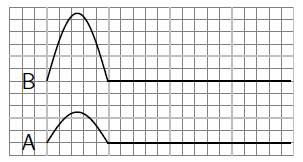
\includegraphics[width=300px]{col11305.imgs/m38801_PG10C4_004.png} % m38801;PG10C4\_004.png;;;6.0;8.5;
        
      \vspace{2pt}
    \vspace{.1in}
    
    \end{center}

 \end{figure}   

    \addtocounter{footnote}{-0}
            \end{enumerate}
        
        

      
    
  \label{m38801**end}
          
\par \raisebox{-5 pt}{
\includegraphics[width=0.5cm]{col11305.imgs/summary_www.png}} Find the answers with the shortcodes:
 \par \begin{tabular}[h]{cccccc}
 (1.) l1f  &  (2.) l1G  &  (3.) l17  &  (4.) l1A  &  (5.) l1o  & \end{tabular}



         \section{ Superposition of pulses}
    \nopagebreak
            \label{m38802} $ \hspace{-5pt}\begin{array}{cccccccccccc}   
\includegraphics[width=0.75cm]{col11305.imgs/summary_fullmarks.png} &   
\includegraphics[width=0.75cm]{col11305.imgs/summary_video.png} &   \end{array} $ \hspace{2 pt}\raisebox{-5 pt}{} {(section shortcode: P10038 )} \par 
    
    
    
    
    
    
  
\label{m38802*fs-id1166232432154}
            \subsection{ Superposition of Pulses}
            \nopagebreak
            
      
      \label{m38802*id316136}Two or more pulses can pass through the same medium at that same time in the same place. When they do they interact with each other to form a different disturbance at that point. The resulting pulse is obtained by using the \textsl{principle of superposition}. The principle of superposition states that the effect of the different pulses is the sum of their individual effects. After pulses pass through each other, each pulse continues along its original direction of travel, and their original amplitudes remain unchanged.\par 
      \label{m38802*id316148}Constructive interference takes place when two pulses meet each other to create a larger pulse. The amplitude of the resulting pulse is the sum of the amplitudes of the two initial pulses. This is shown in Figure~6.5.\par 
\label{m38802*fhsst!!!underscore!!!id567}\begin{definition}
	  \begin{tabular*}{15 cm}{m{15 mm}m{}}
	\hspace*{-50pt}  
\includegraphics[width=0.5in]{col11305.imgs/psflag2.png}   & \Definition{   \label{id2436281}\textbf{ Constructive interference}} { \label{m38802*meaningfhsst!!!underscore!!!id567}
      Constructive interference is when two pulses meet, resulting in a bigger pulse. 
       } 
      \end{tabular*}
      \end{definition}

      
    \setcounter{subfigure}{0}


	\begin{figure}[H] % horizontal\label{m38802*uid53}
    \begin{center}
    \rule[.1in]{\figurerulewidth}{.005in} \\
        \label{m38802*uid53!!!underscore!!!media}\label{m38802*uid53!!!underscore!!!printimage}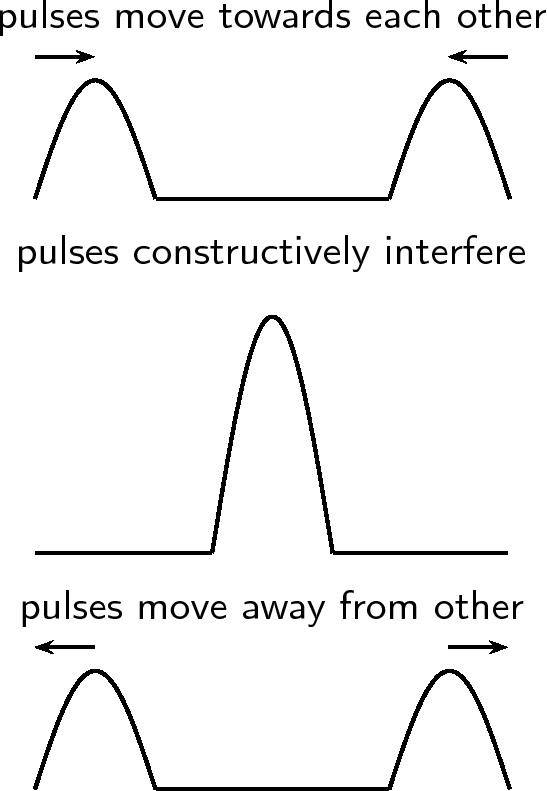
\includegraphics[height=300px]{col11305.imgs/m38802_PG10C4_018.png} % m38802;PG10C4\_018.png;;;6.0;8.5;
        
      \vspace{2pt}
    \vspace{\rubberspace}\par \begin{cnxcaption}
	  \small \textbf{Figure 6.5: }Superposition of two pulses: constructive interference.
	\end{cnxcaption}
      
    \vspace{.1in}
    \rule[.1in]{\figurerulewidth}{.005in} \\
        
    \end{center}

 \end{figure}   

    \addtocounter{footnote}{-0}
    
      \label{m38802*id316190}Destructive interference takes place when two pulses meet and cancel each other. The amplitude of the resulting pulse is the sum of the amplitudes of the two initial pulses, but the one amplitude will be a negative number. This is shown in Figure~6.6. In general, amplitudes of individual pulses add together to give the amplitude of the resultant pulse.\par 
\label{m38802*fhsst!!!underscore!!!id578}\begin{definition}
	  \begin{tabular*}{15 cm}{m{15 mm}m{}}
	\hspace*{-50pt}  
\includegraphics[width=0.5in]{col11305.imgs/psflag2.png}   & \Definition{   \label{id2436357}\textbf{ Destructive interference}} { \label{m38802*meaningfhsst!!!underscore!!!id578}
      Destructive interference is when two pulses meet, resulting in a smaller pulse. 
       } 
      \end{tabular*}
      \end{definition}

      
    \setcounter{subfigure}{0}


	\begin{figure}[H] % horizontal\label{m38802*uid54}
    \begin{center}
    \rule[.1in]{\figurerulewidth}{.005in} \\
        \label{m38802*uid54!!!underscore!!!media}\label{m38802*uid54!!!underscore!!!printimage}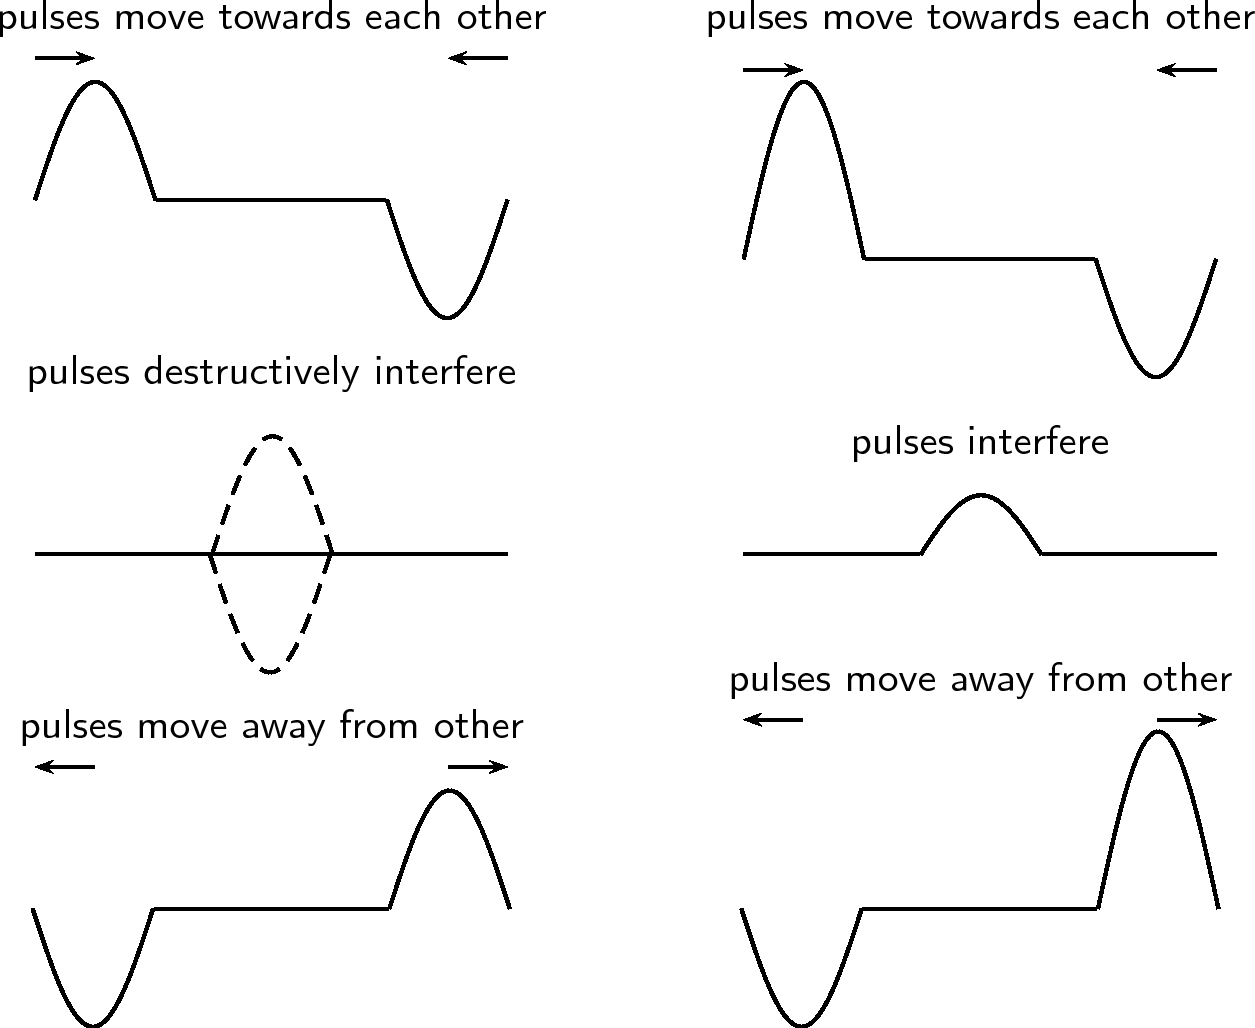
\includegraphics[width=300px]{col11305.imgs/m38802_PG10C4_019.png} % m38802;PG10C4\_019.png;;;6.0;8.5;
        
      \vspace{2pt}
    \vspace{\rubberspace}\par \begin{cnxcaption}
	  \small \textbf{Figure 6.6: }Superposition of two pulses. The left-hand series of images demonstrates destructive interference, since the pulses cancel each other. The right-hand series of images demonstrate a partial cancelation of two pulses, as their amplitudes are not the same in magnitude.
	\end{cnxcaption}
      
    \vspace{.1in}
    \rule[.1in]{\figurerulewidth}{.005in} \\
        
    \end{center}

 \end{figure}   

    \addtocounter{footnote}{-0}
    
\par
            \label{m38802*secfhsst!!!underscore!!!id588}\vspace{.5cm} 
      
      \noindent
      \hspace*{-30pt}
\includegraphics[width=0.5in]{col11305.imgs/pspencil2.png}   \raisebox{25mm}{   
      \begin{mdframed}[linewidth=4, leftmargin=40, rightmargin=40]  
      \begin{exercise}
    \noindent\textbf{Exercise 6.2:  Superposition of Pulses }
      \label{m38802*probfhsst!!!underscore!!!id589}
      \label{m38802*id316249}The two pulses shown below approach each other at \begin{math}1\phantom{\rule{2pt}{0ex}}\mathrm{m}\ensuremath{\cdot}\mathrm{s}{}^{-1}\end{math}. Draw what the waveform would look like after \begin{math}1\phantom{\rule{2pt}{0ex}}\mathrm{s}\end{math}, \begin{math}2\phantom{\rule{2pt}{0ex}}\mathrm{s}\end{math} and \begin{math}5\phantom{\rule{2pt}{0ex}}\mathrm{s}\end{math}.\par 
      \label{m38802*id316283}
        
    \setcounter{subfigure}{0}


	\begin{figure}[H] % horizontal\label{m38802*id316286}
    \begin{center}
    \label{m38802*id316286!!!underscore!!!media}\label{m38802*id316286!!!underscore!!!printimage}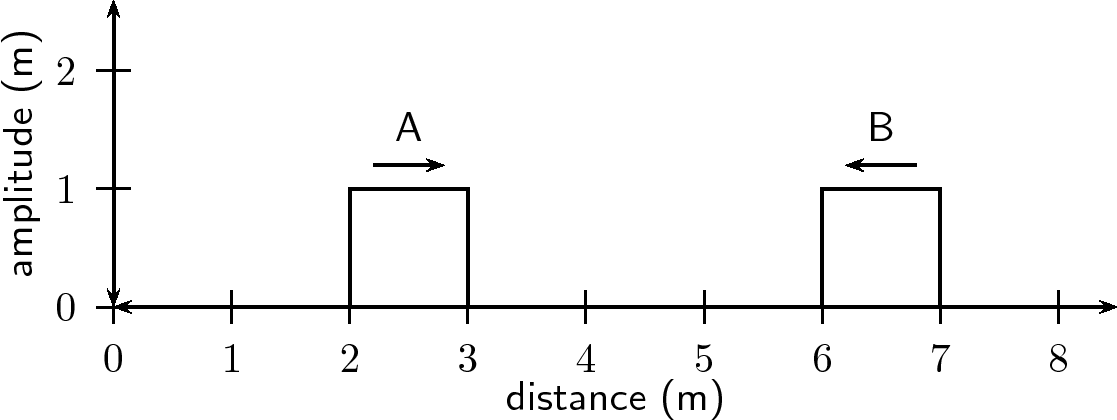
\includegraphics[width=300px]{col11305.imgs/m38802_PG10C4_020.png} % m38802;PG10C4\_020.png;;;6.0;8.5;
        
      \vspace{2pt}
    \vspace{.1in}
    
    \end{center}

 \end{figure}   

    \addtocounter{footnote}{-0}
    
      \par 
      
      \vspace{5pt}
      \label{m38802*solfhsst!!!underscore!!!id601}\noindent\textbf{Solution to Exercise } \label{m38802*listfhsst!!!underscore!!!id601}\begin{enumerate}[noitemsep, label=\textbf{Step} \textbf{\arabic*}. ] 
            \leftskip=20pt\rightskip=\leftskip\item  
      \label{m38802*id316313}After \begin{math}1\phantom{\rule{2pt}{0ex}}\mathrm{s}\end{math}, pulse A has moved \begin{math}1\phantom{\rule{2pt}{0ex}}\mathrm{m}\end{math} to the right and pulse B has moved \begin{math}1\phantom{\rule{2pt}{0ex}}\mathrm{m}\end{math} to the left.\par 
      \label{m38802*id316318}
        
    \setcounter{subfigure}{0}


	\begin{figure}[H] % horizontal\label{m38802*id316321}
    \begin{center}
    \label{m38802*id316321!!!underscore!!!media}\label{m38802*id316321!!!underscore!!!printimage}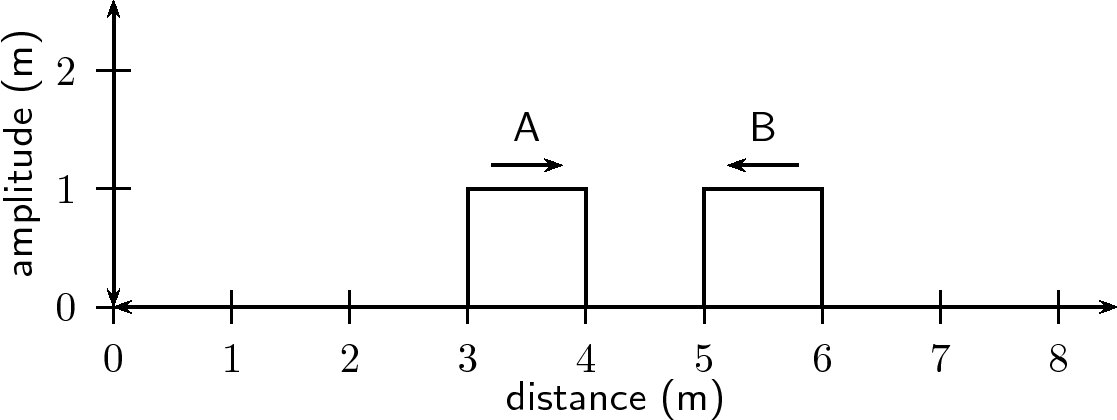
\includegraphics{col11305.imgs/m38802_PG10C4_021.png} % ;PG10C4\_021.png;;;6.0;8.5;
        
      \vspace{2pt}
    \vspace{.1in}
    
    \end{center}

 \end{figure}   

    \addtocounter{footnote}{-0}
    
      \par 
      \item  
      \label{m38802*id316332}After \begin{math}1\phantom{\rule{2pt}{0ex}}\mathrm{s}\end{math} more, pulse A has moved \begin{math}1\phantom{\rule{2pt}{0ex}}\mathrm{m}\end{math} to the right and pulse B has moved \begin{math}1\phantom{\rule{2pt}{0ex}}\mathrm{m}\end{math} to the left.\par 
      \label{m38802*id316337}
        
    \setcounter{subfigure}{0}


	\begin{figure}[H] % horizontal\label{m38802*id316340}
    \begin{center}
    \label{m38802*id316340!!!underscore!!!media}\label{m38802*id316340!!!underscore!!!printimage}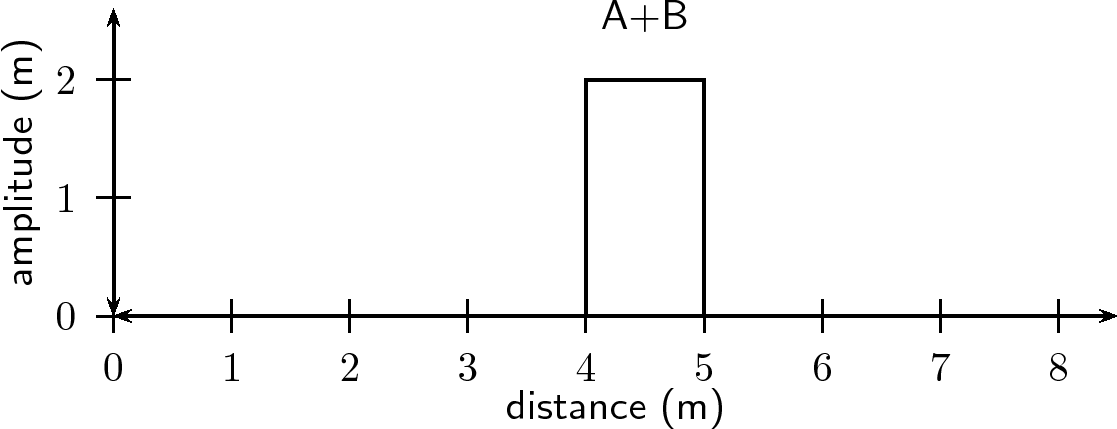
\includegraphics{col11305.imgs/m38802_PG10C4_022.png} % ;PG10C4\_022.png;;;6.0;8.5;
        
      \vspace{2pt}
    \vspace{.1in}
    
    \end{center}

 \end{figure}   

    \addtocounter{footnote}{-0}
    
      \par 
      \item  
      \label{m38802*id316351}After \begin{math}5\phantom{\rule{2pt}{0ex}}\mathrm{s}\end{math}, pulse A has moved \begin{math}5\phantom{\rule{2pt}{0ex}}\mathrm{m}\end{math} to the right and pulse B has moved \begin{math}5\phantom{\rule{2pt}{0ex}}\mathrm{m}\end{math} to the left.\par 
      \label{m38802*id316356}
        
    \setcounter{subfigure}{0}


	\begin{figure}[H] % horizontal\label{m38802*id316360}
    \begin{center}
    \label{m38802*id316360!!!underscore!!!media}\label{m38802*id316360!!!underscore!!!printimage}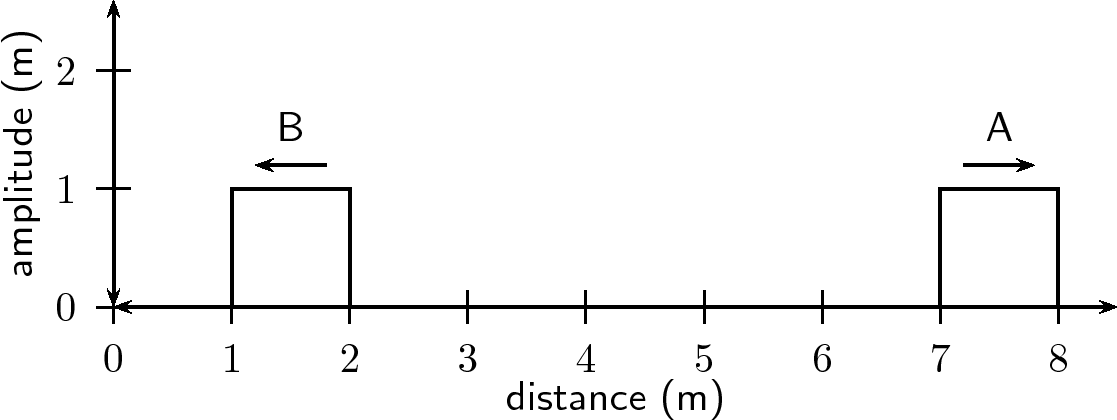
\includegraphics{col11305.imgs/m38802_PG10C4_023.png} % ;PG10C4\_023.png;;;6.0;8.5;
        
      \vspace{2pt}
    \vspace{.1in}
    
    \end{center}

 \end{figure}   

    \addtocounter{footnote}{-0}
    
      \par 
      
      \end{enumerate}
         

    \end{exercise}
    \end{mdframed}
    }
    \noindent
  
\label{m38802*notfhsst!!!underscore!!!id635}
\begin{tabular}{cc}
	   \hspace*{-50pt}\raisebox{-8 mm}{ 
\includegraphics[width=0.5in]{col11305.imgs/pstip2.png}  }& 

	\begin{minipage}{0.85\textwidth}
	\begin{note}
      {tip: }The idea of superposition is one that occurs often in physics. You will see \textsl{much, much more} of superposition!
	\end{note}
	\end{minipage}
	\end{tabular}
	\par
      
\label{m38802*eip-791}
            \subsubsection{ Experiment: Constructive and destructive interference}
            \nopagebreak
            \label{m38802*eip-260}\noindent{}\textbf{Aim}
To demonstrate constructive and destructive interference
\par 
\label{m38802*eip7241}\noindent{}\textbf{Apparatus}Ripple tank apparatus

    \setcounter{subfigure}{0}


	\begin{figure}[H] % horizontal\label{m38802*id63458}
    \begin{center}
    \label{m38802*id63458!!!underscore!!!media}\label{m38802*id63458!!!underscore!!!printimage}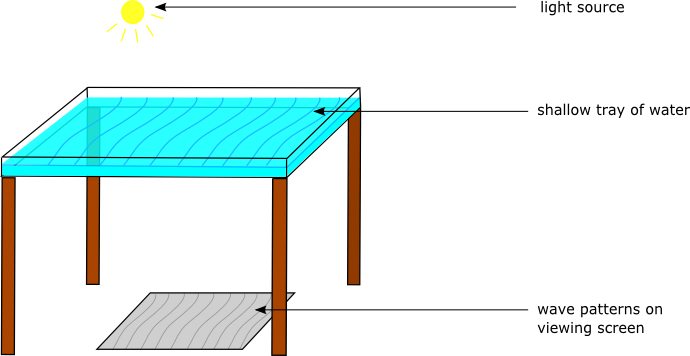
\includegraphics{col11305.imgs/m38802_rippletray.png} % m38802;rippletray.png;;;6.0;8.5;
        
      \vspace{2pt}
    \vspace{.1in}
    
    \end{center}

 \end{figure}   

    \addtocounter{footnote}{-0}
    \par 
\label{m38802*eip7474}\noindent{}\textbf{Method}
\label{m38802*id6242}\begin{enumerate}[noitemsep, label=\textbf{\arabic*}. ] 
            \item Set up the ripple tank\item Produce a single pulse and observe what happens\item Produce two pulses simultaneously and observe what happens\item Produce two pulses at slightly different times and observe what happens\end{enumerate}
        
\par 
\label{m38802*id614134}\noindent{}\textbf{Results and conclusion}
You should observe that when you produce two pulses simultaneously you see them interfere constructively and when you produce two pulses at slightly different times you see them interfere destructively.
\par \label{m38802*secfhsst!!!underscore!!!id636}
            \subsubsection{ Problems Involving Superposition of Pulses }
            \nopagebreak
            \label{m38802*id316401}\begin{enumerate}[noitemsep, label=\textbf{\arabic*}. ] 
            \label{m38802*uid55}\item For the following pulse, draw the resulting wave forms after \begin{math}1\phantom{\rule{2pt}{0ex}}\mathrm{s}\end{math}, \begin{math}2\phantom{\rule{2pt}{0ex}}\mathrm{s}\end{math}, \begin{math}3\phantom{\rule{2pt}{0ex}}\mathrm{s}\end{math}, \begin{math}4\phantom{\rule{2pt}{0ex}}\mathrm{s}\end{math} and \begin{math}5\phantom{\rule{2pt}{0ex}}\mathrm{s}\end{math}. Each pulse is travelling at \begin{math}1\phantom{\rule{2pt}{0ex}}\mathrm{m}\ensuremath{\cdot}\mathrm{s}{}^{-1}\end{math}. Each block represents \begin{math}1\phantom{\rule{2pt}{0ex}}\mathrm{m}\end{math}. The pulses are shown as thick black lines and the undisplaced medium as dashed lines.

    \setcounter{subfigure}{0}


	\begin{figure}[H] % horizontal\label{m38802*id316460}
    \begin{center}
    \label{m38802*id316460!!!underscore!!!media}\label{m38802*id316460!!!underscore!!!printimage}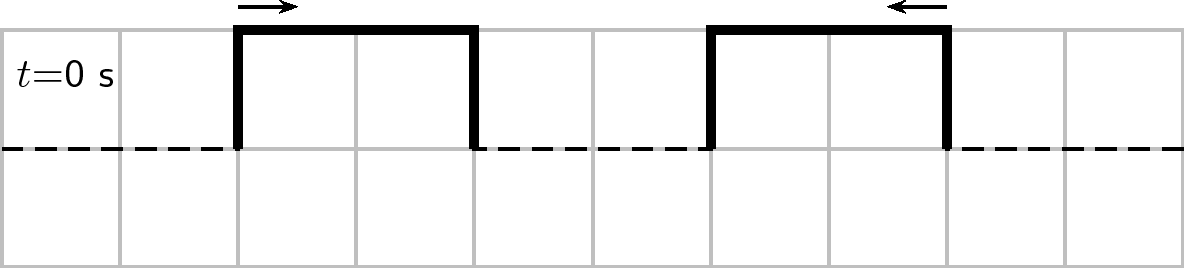
\includegraphics[width=300px]{col11305.imgs/m38802_PG10C4_024.png} % m38802;PG10C4\_024.png;;;6.0;8.5;
        
      \vspace{2pt}
    \vspace{.1in}
    
    \end{center}

 \end{figure}   

    \addtocounter{footnote}{-0}
            \label{m38802*uid57}\item For the following pulse, draw the resulting wave forms after \begin{math}1\phantom{\rule{2pt}{0ex}}\mathrm{s}\end{math}, \begin{math}2\phantom{\rule{2pt}{0ex}}\mathrm{s}\end{math}, \begin{math}3\phantom{\rule{2pt}{0ex}}\mathrm{s}\end{math}, \begin{math}4\phantom{\rule{2pt}{0ex}}\mathrm{s}\end{math} and \begin{math}5\phantom{\rule{2pt}{0ex}}\mathrm{s}\end{math}. Each pulse is travelling at \begin{math}1\phantom{\rule{2pt}{0ex}}\mathrm{m}\ensuremath{\cdot}\mathrm{s}{}^{-1}\end{math}. Each block represents \begin{math}1\phantom{\rule{2pt}{0ex}}\mathrm{m}\end{math}. The pulses are shown as thick black lines and the undisplaced medium as dashed lines.
    \setcounter{subfigure}{0}


	\begin{figure}[H] % horizontal\label{m38802*id316477}
    \begin{center}
    \label{m38802*id316477!!!underscore!!!media}\label{m38802*id316477!!!underscore!!!printimage}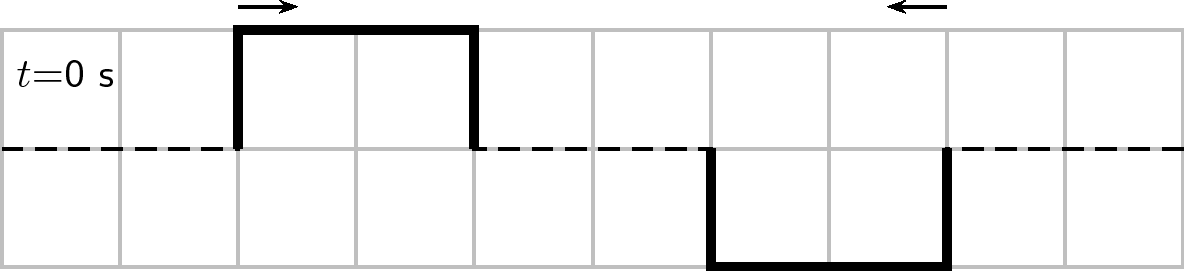
\includegraphics[width=300px]{col11305.imgs/m38802_PG10C4_025.png} % m38802;PG10C4\_025.png;;;6.0;8.5;
        
      \vspace{2pt}
    \vspace{.1in}
    
    \end{center}

 \end{figure}   

    \addtocounter{footnote}{-0}
            \label{m38802*uid58}\item For the following pulse, draw the resulting wave forms after \begin{math}1\phantom{\rule{2pt}{0ex}}\mathrm{s}\end{math}, \begin{math}2\phantom{\rule{2pt}{0ex}}\mathrm{s}\end{math}, \begin{math}3\phantom{\rule{2pt}{0ex}}\mathrm{s}\end{math}, \begin{math}4\phantom{\rule{2pt}{0ex}}\mathrm{s}\end{math} and \begin{math}5\phantom{\rule{2pt}{0ex}}\mathrm{s}\end{math}. Each pulse is travelling at \begin{math}1\phantom{\rule{2pt}{0ex}}\mathrm{m}\ensuremath{\cdot}\mathrm{s}{}^{-1}\end{math}. Each block represents \begin{math}1\phantom{\rule{2pt}{0ex}}\mathrm{m}\end{math}. The pulses are shown as thick black lines and the undisplaced medium as dashed lines.
    \setcounter{subfigure}{0}


	\begin{figure}[H] % horizontal\label{m38802*id316495}
    \begin{center}
    \label{m38802*id316495!!!underscore!!!media}\label{m38802*id316495!!!underscore!!!printimage}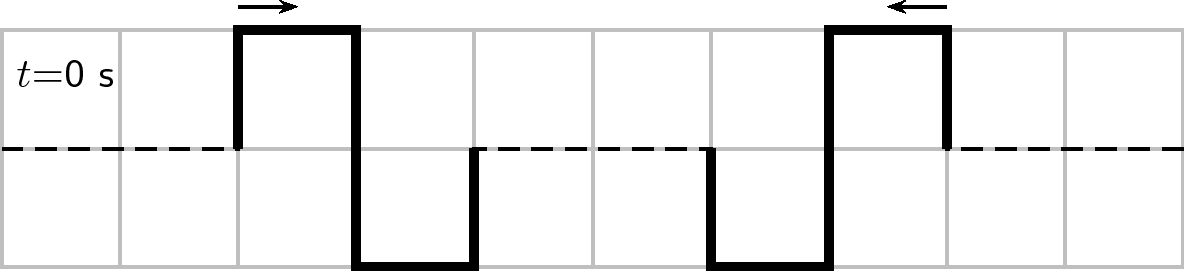
\includegraphics[width=300px]{col11305.imgs/m38802_PG10C4_026.png} % m38802;PG10C4\_026.png;;;6.0;8.5;
        
      \vspace{2pt}
    \vspace{.1in}
    
    \end{center}

 \end{figure}   

    \addtocounter{footnote}{-0}
            \label{m38802*uid59}\item For the following pulse, draw the resulting wave forms after \begin{math}1\phantom{\rule{2pt}{0ex}}\mathrm{s}\end{math}, \begin{math}2\phantom{\rule{2pt}{0ex}}\mathrm{s}\end{math}, \begin{math}3\phantom{\rule{2pt}{0ex}}\mathrm{s}\end{math}, \begin{math}4\phantom{\rule{2pt}{0ex}}\mathrm{s}\end{math} and \begin{math}5\phantom{\rule{2pt}{0ex}}\mathrm{s}\end{math}. Each pulse is travelling at \begin{math}1\phantom{\rule{2pt}{0ex}}\mathrm{m}\ensuremath{\cdot}\mathrm{s}{}^{-1}\end{math}. Each block represents \begin{math}1\phantom{\rule{2pt}{0ex}}\mathrm{m}\end{math}. The pulses are shown as thick black lines and the undisplaced medium as dashed lines.
    \setcounter{subfigure}{0}


	\begin{figure}[H] % horizontal\label{m38802*id316512}
    \begin{center}
    \label{m38802*id316512!!!underscore!!!media}\label{m38802*id316512!!!underscore!!!printimage}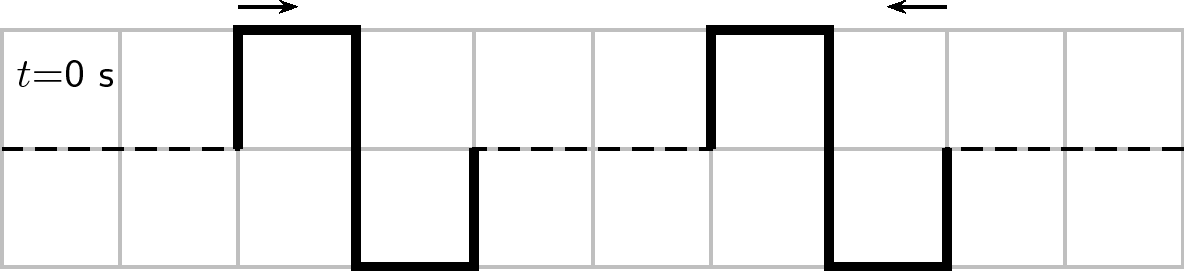
\includegraphics[width=300px]{col11305.imgs/m38802_PG10C4_027.png} % m38802;PG10C4\_027.png;;;6.0;8.5;
        
      \vspace{2pt}
    \vspace{.1in}
    
    \end{center}

 \end{figure}   

    \addtocounter{footnote}{-0}
            \label{m38802*uid60}\item For the following pulse, draw the resulting wave forms after \begin{math}1\phantom{\rule{2pt}{0ex}}\mathrm{s}\end{math}, \begin{math}2\phantom{\rule{2pt}{0ex}}\mathrm{s}\end{math}, \begin{math}3\phantom{\rule{2pt}{0ex}}\mathrm{s}\end{math}, \begin{math}4\phantom{\rule{2pt}{0ex}}\mathrm{s}\end{math} and \begin{math}5\phantom{\rule{2pt}{0ex}}\mathrm{s}\end{math}. Each pulse is travelling at \begin{math}1\phantom{\rule{2pt}{0ex}}\mathrm{m}\ensuremath{\cdot}\mathrm{s}{}^{-1}\end{math}. Each block represents \begin{math}1\phantom{\rule{2pt}{0ex}}\mathrm{m}\end{math}. The pulses are shown as thick black lines and the undisplaced medium as dashed lines.
    \setcounter{subfigure}{0}


	\begin{figure}[H] % horizontal\label{m38802*id316530}
    \begin{center}
    \label{m38802*id316530!!!underscore!!!media}\label{m38802*id316530!!!underscore!!!printimage}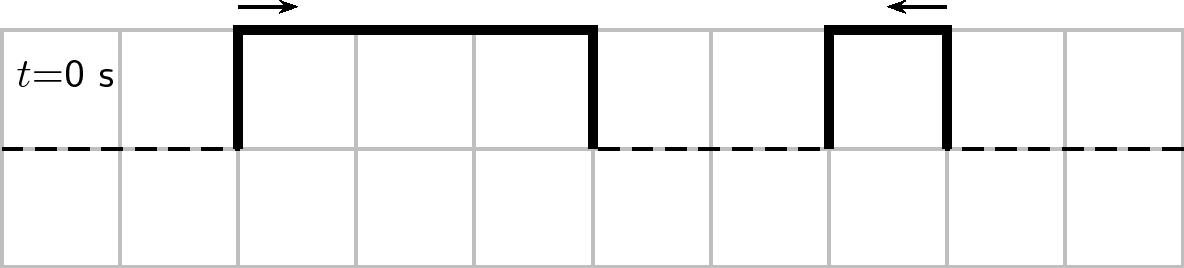
\includegraphics[width=300px]{col11305.imgs/m38802_PG10C4_028.png} % m38802;PG10C4\_028.png;;;6.0;8.5;
        
      \vspace{2pt}
    \vspace{.1in}
    
    \end{center}

 \end{figure}   

    \addtocounter{footnote}{-0}
            \label{m38802*uid61}\item For the following pulse, draw the resulting wave forms after \begin{math}1\phantom{\rule{2pt}{0ex}}\mathrm{s}\end{math}, \begin{math}2\phantom{\rule{2pt}{0ex}}\mathrm{s}\end{math}, \begin{math}3\phantom{\rule{2pt}{0ex}}\mathrm{s}\end{math}, \begin{math}4\phantom{\rule{2pt}{0ex}}\mathrm{s}\end{math} and \begin{math}5\phantom{\rule{2pt}{0ex}}\mathrm{s}\end{math}. Each pulse is travelling at \begin{math}1\phantom{\rule{2pt}{0ex}}\mathrm{m}\ensuremath{\cdot}\mathrm{s}{}^{-1}\end{math}. Each block represents \begin{math}1\phantom{\rule{2pt}{0ex}}\mathrm{m}\end{math}. The pulses are shown as thick black lines and the undisplaced medium as dashed lines.
    \setcounter{subfigure}{0}


	\begin{figure}[H] % horizontal\label{m38802*id316547}
    \begin{center}
    \label{m38802*id316547!!!underscore!!!media}\label{m38802*id316547!!!underscore!!!printimage}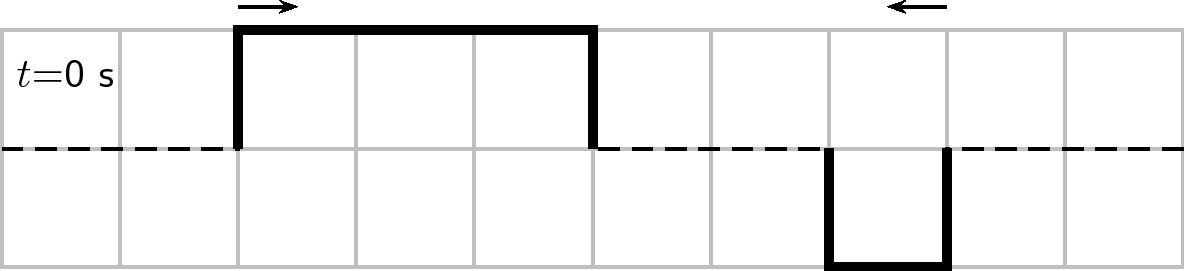
\includegraphics[width=300px]{col11305.imgs/m38802_PG10C4_029.png} % m38802;PG10C4\_029.png;;;6.0;8.5;
        
      \vspace{2pt}
    \vspace{.1in}
    
    \end{center}

 \end{figure}   

    \addtocounter{footnote}{-0}
            \label{m38802*uid62}\item 
          What is superposition of waves?\newline
            
\label{m38802*uid64}\item What is constructive interference?\newline
            
\label{m38802*uid65}\item What is destructive interference?\newline
            
        \end{enumerate}
        
      

    

\label{m38802*fs-id1165499443114} The following presentation provides a summary of the work covered in this chapter. Although the presentation is titled waves, the presentation covers pulses only.
      
    \setcounter{subfigure}{0}


	\begin{figure}[H] % horizontal\label{m38802*slidesharefigure}
    
    \label{m38802*slidesharemedia}\label{m38802*slideshareflash}\raisebox{-5 pt}{ 
\includegraphics[width=0.5cm]{col11305.imgs/summary_www.png}} { (Presentation:  P10039 )}
      
      \vspace{2pt}
    \vspace{.1in}
    
    

 \end{figure}   

    \addtocounter{footnote}{-0}
    
\par 
  \label{m38802*eip-812}
\par \raisebox{-5 pt}{
\includegraphics[width=0.5cm]{col11305.imgs/summary_www.png}} Find the answers with the shortcodes:
 \par \begin{tabular}[h]{cccccc}
 (1.) l1M  &  (2.) l1e  &  (3.) l1t  &  (4.) l1z  &  (5.) l1u  &  (6.) l1J  &  (7.) l1S  &  (8.) l1h  &  (9.) lrg  & \end{tabular}



            \subsection{ Summary}
            \nopagebreak
            \label{m38802*eip-404}\begin{itemize}[noitemsep]
            \item A medium is the substance or material in which a wave will move\item A pulse is a single disturbance that moves through a medium\item The amplitude of a pules is a measurement of how far the medium is displaced from rest\item Pulse speed is the distance a pulse travels per unit time\item Constructive interference is when two pulses meet and result in a bigger pulse\item Destructive interference is when two pulses meet and and result in a smaller pulse\item We can draw graphs to show the motion of a particle in the medium or to show the motion of a pulse through the medium\item When a pulse moves from a thin rope to a thick rope, the speed and pulse length decrease. The pulse will be reflected and inverted in the thin rope. The reflected pulse has the same length and speed, but a different amplitude\item When a pulse moves from a thick rope to a thin rope, the speed and pulse length increase. The pulse will be reflected in the thick rope. The reflected pulse has the same length and speed, but a different amplitude\item A pulse reaching a free end will be reflected but not inverted. A pulse reaching a fixed end will be reflected and inverted\end{itemize}
        \label{m38802*cid9}
            \subsection{ Exercises - Transverse Pulses}
            \nopagebreak
            
      
      \label{m38802*id316647}\begin{enumerate}[noitemsep, label=\textbf{\arabic*}. ] 
            \label{m38802*uid66}\item A heavy rope is flicked upwards, creating a single pulse in the rope. Make a drawing of the rope and indicate the following in your drawing:
\label{m38802*id316663}\begin{enumerate}[noitemsep, label=\textbf{\alph*}. ] 
            \label{m38802*uid67}\item The direction of motion of the pulse
\label{m38802*uid68}\item Amplitude
\label{m38802*uid69}\item Pulse length
\label{m38802*uid70}\item Position of rest
\end{enumerate}
                \label{m38802*uid71}\item A pulse has a speed of \begin{math}2,5\phantom{\rule{2pt}{0ex}}\mathrm{m}\ensuremath{\cdot}\mathrm{s}{}^{-1}\end{math}. How far will it have travelled in \begin{math}6\phantom{\rule{2pt}{0ex}}\mathrm{s}\end{math}?\newline
            
\label{m38802*uid72}\item A pulse covers a distance of \begin{math}75\phantom{\rule{2pt}{0ex}}\mathrm{cm}\end{math} in \begin{math}2,5\phantom{\rule{2pt}{0ex}}\mathrm{s}\end{math}. What is the speed of the pulse?\newline
            
\label{m38802*uid73}\item How long does it take a pulse to cover a distance of \begin{math}200\phantom{\rule{2pt}{0ex}}\mathrm{mm}\end{math} if its speed is \begin{math}4\phantom{\rule{2pt}{0ex}}\mathrm{m}\ensuremath{\cdot}\mathrm{s}{}^{-1}\end{math}?\newline
            
\label{m38802*uid74}\item The following position-time graph for a pulse in a slinky spring is given. Draw an accurate sketch graph of the velocity of the pulse against time.

    \setcounter{subfigure}{0}


	\begin{figure}[H] % horizontal\label{m38802*id316803}
    \begin{center}
    \label{m38802*id316803!!!underscore!!!media}\label{m38802*id316803!!!underscore!!!printimage}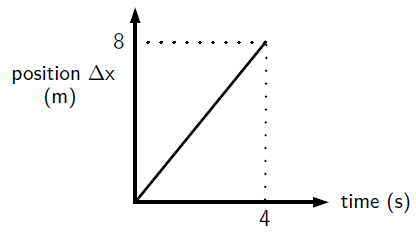
\includegraphics{col11305.imgs/m38802_PG10C4_030.png} % m38802;PG10C4\_030.png;;;6.0;8.5;
        
      \vspace{2pt}
    \vspace{.1in}
    
    \end{center}

 \end{figure}   

    \addtocounter{footnote}{-0}
            \label{m38802*uid75}\item The following velocity-time graph for a particle in a medium is given. Draw an accurate sketch graph of the position of the particle vs. time.

    \setcounter{subfigure}{0}


	\begin{figure}[H] % horizontal\label{m38802*id316826}
    \begin{center}
    \label{m38802*id316826!!!underscore!!!media}\label{m38802*id316826!!!underscore!!!printimage}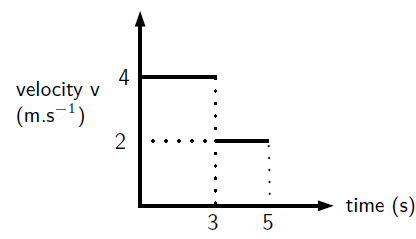
\includegraphics{col11305.imgs/m38802_PG10C4_031.png} % m38802;PG10C4\_031.png;;;6.0;8.5;
        
      \vspace{2pt}
    \vspace{.1in}
    
    \end{center}

 \end{figure}   

    \addtocounter{footnote}{-0}
            \label{m38802*uid76}\item Describe what happens to a pulse in a slinky spring when:
\label{m38802*id316845}\begin{enumerate}[noitemsep, label=\textbf{\alph*}. ] 
            \label{m38802*uid77}\item the slinky spring is tied to a wall.
\label{m38802*uid78}\item the slinky spring is loose, i.e. not tied to a wall.
\end{enumerate}
        
(Draw diagrams to explain your answers.)\newline
            
\label{m38802*uid79}\item The following diagrams each show two approaching pulses. Redraw the diagrams to show what type of interference takes place, and label the type of interference.
\label{m38802*id316891}\begin{enumerate}[noitemsep, label=\textbf{\alph*}. ] 
            \label{m38802*uid80}\item 
    \setcounter{subfigure}{0}


	\begin{figure}[H] % horizontal\label{m38802*id316905}
    \begin{center}
    \label{m38802*id316905!!!underscore!!!media}\label{m38802*id316905!!!underscore!!!printimage}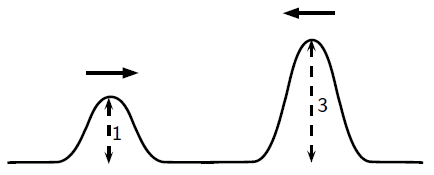
\includegraphics{col11305.imgs/m38802_PG10C4_032.png} % m38802;PG10C4\_032.png;;;6.0;8.5;
        
      \vspace{2pt}
    \vspace{.1in}
    
    \end{center}

 \end{figure}   

    \addtocounter{footnote}{-0}
    \label{m38802*uid81}\item 
    \setcounter{subfigure}{0}


	\begin{figure}[H] % horizontal\label{m38802*id316923}
    \begin{center}
    \label{m38802*id316923!!!underscore!!!media}\label{m38802*id316923!!!underscore!!!printimage}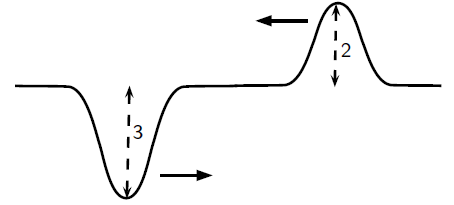
\includegraphics{col11305.imgs/m38802_PG10C4_033.png} % m38802;PG10C4\_033.png;;;6.0;8.5;
        
      \vspace{2pt}
    \vspace{.1in}
    
    \end{center}

 \end{figure}   

    \addtocounter{footnote}{-0}
    \end{enumerate}
                \label{m38802*uid82}\item Two pulses, A and B, of identical shape and amplitude are simultaneously generated in two identical wires of equal mass and length. Wire A is, however, pulled tighter than wire B. Which pulse will arrive at the other end first, or will they both arrive at the same time?\newline
            
\end{enumerate}
        
    

  \label{m38802**end}
          
       
    
  \label{21d48a6f8839b4b265192acd9ea3d978**end}
    
\par \raisebox{-5 pt}{
\includegraphics[width=0.5cm]{col11305.imgs/summary_www.png}} Find the answers with the shortcodes:
 \par \begin{tabular}[h]{cccccc}
 (1.) lrl  &  (2.) lri  &  (3.) lr3  &  (4.) lrO  &  (5.) lrc  &  (6.) lrx  &  (7.) lra  &  (8.) lrC  &  (9.) lr1  & \end{tabular}



